\chapter{Bootstrap Percolation on the Hamming Torus}
\label{chap:bootstrap}

\section{Introduction}

 \newcommand{\note}[1]{{\bf \textcolor{blue}
{[#1\marginpar{\textcolor{red}{***}}]}}}
\newcommand{\bfit}[1]
{\emph{\textbf{#1}}}

Bootstrap percolation is a simple growth model, introduced to understand nucleation and metastability in physical processes such as crack formations, clustering, and alignment of magnetic
spins. It was introduced in 1979 by Chalupa, Leath and Reich \cite{bethe}. For more applications and background see surveys by Adler and Levi \cite{brazil} and Holroyd~\cite{holroyd-survey}.

Given a graph $G=(V,E)$, {\it bootstrap percolation\/} with {\it threshold\/} $\threshold$
is the following discrete-time growth process: given an initial configuration $\omega \in
\{0,1\}^V$, an increasing sequence of configurations 
$\omega=\omega_0,\omega_1,\ldots$ is defined by
$$
\omega_{j+1}(v)=
\begin{cases}
1& \text{if $\omega_j(v)=1$ or $\sum_{w \sim  v}\omega_j(w) \geq
\threshold$}\\
0 &\text{else}
\end{cases}
$$
and $\omega_\infty$ is the pointwise limit of $\omega_j$ as $j\to\infty$.
The initial configuration $\omega$ is random; $\{\omega(v): v \in V\}$ is a collection of i.i.d.\ Bernoulli random variables with parameter $p$. A natural quantity to study is $\prob_{p}(\omega_\infty\equiv 1)$. Indeed, first results in this area were by van Enter~\cite{vanenter} and Schonmann~\cite{schonmann}, who proved that for the lattice $\mathbb{Z}^d$ this probability is either 1 or 0 according to whether $\threshold \le d$ or $\threshold > d$. Following the seminal work of Aizenman and Lebowitz~\cite{aizenman},
%who studied bootstrap percolation on large cubes in $\mathbb{Z}^d$
it became clear that this process is even more interesting on large {\em finite} graphs.  For a family of graphs depending on a single parameter $n$, with the number of vertices going to infinity as $n$ increases, we assume that $p=p(n)$, and study the dependence on $n$ of the critical probability~$p_c$ defined by
\begin{equation*}
\prob_{p_c}(\omega_\infty\equiv1)=1/2.
\end{equation*}

We mention only a few prominent results on how $p_c$ scales with $n$. Let $[n]=\{1,\dots,n\}$. For a large lattice cube $[n]^d\subset \mathbb{Z}^d$
(where each point is connected to the nearest $2d$ points) , Aizenman and Lebowitz \cite{aizenman} proved that $p_c$ behaves as $(\frac{1}{\log n})^{d-1}$ when $\threshold=2$, and later Cerf and Cirillo~\cite{cerfcirillo} and Cerf and Manzo~\cite{cerfmanzo} established the scaling $(\log_{\threshold-1} n)^{-d+\threshold-1}$ for $3\le \theta\le d$; here $\log_{\threshold-1}$ denotes the $(\theta-1)$'st iteration of the logarithm. For the hypercube $\{0,1\}^n$,
 Balogh and Bollob\'as~\cite{BB:2006} proved that the scaling 
for $p_c$ is $n^{-2}4^{-\sqrt n}$ when $\threshold=2$; by contrast,  for the very large threshold 
 $\threshold=\ceil{n/2}$, the {\it majority bootstrap percolation\/} studied by  Balogh, Bollob\'as, and Morris~\cite{bollobas}, 
$p_c$ is close to $1/2$.

Such scaling results do not tell the whole story. They suggest the existence of an {\it order parameter\/}, a function of $p$ and $n$ whose size determines whether $\prob_{p}(\omega_\infty\equiv1)$ is small or close to 1; e.g., on a lattice square $[n]^2$, such a function is $p\log n$. This leads to two natural questions: Does the probability exhibit a sharp jump from 0 to 1 as the order parameter increases? Does the location of the (purported) sharp jump converge as $n$ increases? (There are good reasons to expect the answer to the first question to be positive in surprising generality~\cite{FK:1996}.)

In a major breakthrough, Holroyd~\cite{holroyd} established a positive answer to both questions
in the lattice square case, and proved that $p_c\sim \frac{\pi^2}{18 \log n}$. This celebrated theorem contradicted conjectures based on simulations, which is due to the fact that $p_c\log n$ converges to its limit very slowly, as about $1/\sqrt{\log n}$
%That is if  $p>>( \frac{\pi^2}{18 \log n})(1+1/\sqrt{\log n})$ then $\prob(\omega_\infty=1) \to 1$ and if $p<<( \frac{\pi^2}{18 \log n})(1-1/\sqrt{\log n})$ then $\prob(\omega_\infty=1) \to 0$
~\cite{GGM:2012}. For lattice cubes $[n]^d$, $d\ge 3$ and $2\le \theta\le d$, the sharp transition was established by Balogh, Bollob\'as, Duminil-Copin, and Morris~\cite{bollobas1, bollobas2}.

Besides varying the dimension of the lattice or the threshold, one can also vary the  neighborhood of a point. For example, Holroyd, Liggett and Romik \cite{hlr} consider the lattice square $[n]^2$, with the ``cross'' neighborhood of a point that consists of $k-1$ points in each of the 4 axis directions, and $\threshold=k$. In this case, $p_c\sim\frac{\pi^2}{3k(k+1) \log n}$.

In this paper we consider bootstrap percolation on the {\it Hamming torus\/} (or Hamming graph) with vertex set $V = [n]^d$, where $v\in V$ and $w\in V$ are adjacent iff $v-w$ has exactly one nonzero coordinate.  
%In other words, the Hamming torus is the Cartesian product of $d$ complete graphs $K_n$.  
In $d=2$, this graph could be interpreted as taking the Holroyd-Liggett-Romik neighborhood \cite{hlr} with $k=\infty$. For any $d$, the neighborhood of a point $v$ is the union of all $d$ lines through $v$ parallel to the axes. We emphasize, however, that the threshold $\threshold$ remains fixed as $n$ increases (although some of our results assume that $\threshold$ is large).  Other models of percolation, including bond percolation~\cite{BCHSS:2005, HL:2010} and site percolation~\cite{S:2010}, have been considered on the Hamming torus, and were shown to exhibit interesting behavior due to the large neighborhood sizes relative to nearest-neighbor lattices and hypercubes.  For the same reason, we expect qualitatively different transition phenomena in bootstrap percolation on the Hamming torus from those described above. First, the critical probability is much smaller. In fact, our results suggest that 
$p_c$ is of the order $n^{-\alpha}$, for some critical exponent $\alpha > 1$. We are able to determine $\alpha$ exactly in a few cases, and give estimates otherwise. Moreover, we expect that varying the order parameter $n^{\alpha}p$ does {\it not\/} lead to a sharp jump of $\prob_{p}(\omega_\infty\equiv1)$ from 0 to 1; instead, this probability gradually approaches 0 (resp.~1) as the order parameter approaches 0 (resp.~$\infty$). When $d=2$ this is easy to demonstrate for arbitrary $\threshold$, but when $d\ge 3$ the combinatorics are quite difficult even when $\alpha$ is known exactly. Nevertheless, we succeeded in analyzing the case $d=\theta=3$, which has $\alpha=2$: we give an explicit formula for the limit of $\prob_{p} (\omega_\infty\equiv1)$ when $pn^2=a\in(0,\infty)$.  See \cite{JLTV}, Theorem 3.2, for an analogous result
for bootstrap percolation on Erd\"os-R\`enyi random graphs.


Moreover, in dimensions $d\ge 3$  we find two distinct critical exponents. When $p$ is much smaller than $n^{-1-d/\theta}$, the model does not accomplish much; with high probability it does not even fill a single line. When $p$ is much larger than $n^{-1-d/\theta}$, but smaller than $n^{-1-2/\theta-c'/\threshold^{3/2}}$, for 
 large enough $\theta$, with high probability some lines become open, but no two dimensional subgraphs do, and thus $\prob_{p}(\omega_\infty\equiv1)\to 0$. When $p>n^{-1-2/\theta-c''/\threshold^{3/2}}$, and $\threshold$ is large 
enough,
$\prob_{p}(\omega_\infty\equiv1)\to 1$. Here, $0<c''<c'$ are constants depending on $d$.  
%there are distinct critical exponents for $p_c(2,2,d)$, $p_c(4,2,d)$, \dots , $p_c(2,2k,d)$ for $k<\sqrt{d}$

It remains an open question for $\threshold>2$ whether the critical exponents for the appearance of open subspaces with dimension $i$ are distinct for each $2\leq i \leq d$. However, in subsequent work, Slivken has proven that for $\threshold =2$, there are distinct critical exponents for the appearance of open subspaces with dimension $2i$ for $1\le i < \sqrt{d}$~\cite{slivken}.

%In the next section we give rigorous statements of our results. In the subsequent sections we state (and prove) our %results. \note{More description of what is done where is needed here.}



\section{Statement of Results}
Let $\cF$ be a family of subsets of $[n]^d$. Then
$$\prob_p(\exists F \in \cF:\  \omega_\infty|_F\equiv 1)$$
is a nondecreasing function in $p$. For $\cF_i$ the collection of $i$-dimensional subgraphs of $G$, there exists a threshold function $p_c(i,d)$ such that 
$$\prob_{p_c(i,d)}(\exists F \in \cF_i:\  \omega_\infty|_F\equiv1)=0.5.$$
If $\omega_j(v)=1$ we say $v$ is open at step $j$, and a set $S \subseteq V$ is open if each $v \in S$ is open, 
i.e., $\omega_j|_S\equiv 1$.

%The smaller that $i$ is, the easier it is to calculate $p_c(i,d)$. 
For $i=0$ we have an additional critical probability
$p^*_c(0,d)$. We would like to define it to be the threshold function for  
$\omega_\infty \not\equiv \omega_0$; unfortunately, this is not an increasing
event. Instead, we define the event
$$\abovethresh=\left\{ \exists v: \sum_{w \sim v}\omega_0(w)\geq \threshold \right\}$$
and $p^*_c(0,d)$ to be the $p$ for which $P_p(\abovethresh)=0.5$.


\begin{comment}
We believe that for all $i \geq 1$ and $d$, $p_c$ has the following form. 
\begin{conjecture}
For all $i$ and $d$ and $n$ sufficiently large
$$p_c(i,d)=n^{-1 - \frac{c_1(i,d)}{\threshold} - \frac{c_{3/2}(i,d)}{\threshold^{3/2}}+o(\threshold^{-3/2})}.$$
\end{conjecture}
We make substantial progress to proving that this is the
case for all $i$ and $d$, but in general we are only able to prove that if $n$ is sufficinetly large with $\threshold$ then
$$p_c(i,d)=n^{-1 - \frac{c_1(i,d)}{\threshold} - \theta(\threshold^{-3/2})}.$$
In general for fixed $n,d$ and $i$ we get bounds on the critical $p$, but the precise bounds that we get are quite messy to state. In the rest of this section we put all of our results in a common form. Many of the theorems have are given in a stronger form in the following sections. 
\end{comment}

We write $f(n)\sim g(n)$ if $\frac{f(n)}{g(n)}  \to 1.$ 
%Fix $\threshold, i, d \in \N$ with $i \leq d$. 
We conjecture that for every $\threshold, i, d \in \N$ with $i \leq d$, there exists $a_c=a_c(\theta,i,d)$ and $\alpha_c=\alpha_c(\theta,i,d)$
such that
$$p_c(i,d) \sim a_cn^{-\alpha_c}.$$
Moreover there exists a nondecreasing function $G=G(\theta,i,d):\R^+ \to [0,1]$ such that
$G(x) \to 0$ as $x \to 0$, 
$G(x) \to 1$ as $x \to \infty$, and if $p=a n^{-\alpha_c}$ then
$$\prob_{p}(\exists F \in \cF_i:\  \omega_\infty|_F\equiv1) \sim G(a).$$

We are able to prove that this is the case for $d=2$.
\begin{theorem}
\label{2d-thm}
Let $d=2$, $k = \lceil \threshold/2 \rceil > 1$ and $p=an^{-1-\frac{1}{k}}$. 
Then
$$
\prob( \omega_\infty\equiv 1) \to
\begin{cases}
1-e^{-2a^k/k!}& \text{if $\threshold$ is odd,}
\\
(1-e^{-a^k/k!})^2 &\text{if $\threshold$ is even.}
\end{cases}
$$
Thus
$$p_c(2,2)=p_c(1,2)=p^*_c(0,2)=n^{-1-\frac{2}{\threshold} + o(\threshold^{-3/2})}.$$
Furthermore,
$$\prob\big(\{\omega_\infty \not\equiv \omega_0\} \setminus \{\omega_\infty\equiv 1\}\big)=o(1).$$
\end{theorem}

As $d$ increases the problem becomes more intricate. For $d=3$, we are able to identify the limit under critical scaling when 
$\threshold=3$. 

\begin{theorem}
\label{3d-spanning-thm}
Let $d=3$, $\threshold=3$ and $p = an^{-2}$ with $a>0$.  Then as $n\to \infty$
\begin{equation}
\prob_{p}(\omega_\infty \equiv 1) \to 1 - e^{-a^3 - (3/2)a^2(1-e^{-2a})}\left[\frac{3}{2} a^2\left(\left(e^{-a}+ae^{-3a}\right)^2-e^{-2a}\right)e^{-a^2e^{-2a}} + e^{a^3e^{-3a}} \right].
\end{equation}
\end{theorem}

Other three dimensional results include 
determining the critical exponents $(\beta_c)$ for $d=3$ and low thresholds, but not the exact constants $\alpha_c$; 
see Section 5 for details. 

Many of our results state that
$$p_c(i,d)=n^{-1 - \frac{c_1(i,d)}{\threshold} - \Theta(\threshold^{-3/2})},$$
where $c_1=c_1(i,d)$ is a constant. This shorthand notation means that, for a large 
$n$, we can get a lower bound and and upper boud for $p_c(i,d)$ of the stated form, 
with constants in the correction term $\Theta(\threshold^{-3/2})$ depending on $i$ and $d$.



For general $d\ge 3$, 
we calculate $p_c^*(0,d)$ and $p_c(1,d)$ for all $d\geq 2$ quite
precisely.
\begin{theorem} \label{la liga}
Let $p=f(n)n^{-1-\frac{d}{\threshold}}$ and $d,\threshold \geq 3$.
If $f(n)\to 0$ then $$\prob(\abovethresh) \to 0$$
and
if $f(n)\to \infty$ then $$\prob(\exists \text{ a line $\Ln$ such that } \omega_\infty|_\Ln\equiv1) \to 1.$$
%Thus $c_1(1,d)=d$ and $c_{3/2}(1,d)=0.$
\end{theorem}

Furthermore, we get good bounds on 
$p_c(2,d)$, the threshold for existence of two dimensional subspaces in the final configuration.
\begin{theorem} \label{epl} Fix $d$ and fix $\threshold$ sufficiently large depending on $d$. For $n$ sufficiently large 
$$n^{-1 - \frac{2}{\threshold} - \frac{4d^2 + 3}{\threshold^{3/2}}}
\leq p_c(2,d) \leq
n^{-1 - \frac{2}{\threshold} - \frac{\sqrt{8(d-2.1)}}{\threshold^{3/2}}}.
$$
\end{theorem}
(We have not attempted to optimize the constants $\sqrt{8(d-2.1)}$ and $4d^2 + 3$ in the above theorem.)
The key arguments in the proof of Theorem~\ref{epl} are Lemmas \ref{cajunsprel1} and \ref{2d-span-lb-lem}.

The higher the dimensions $i$ and $d$, 
the more difficult it becomes to calculate $p_c(i,d)$. 
However, Theorems \ref{la liga}  and \ref{epl} are sufficient for us to get bounds on $p_c(i,d)$ for all $i,d \geq 2$.

%%% Fix the \Theta(\threshold)
\begin{theorem}
For all $i\ge 2$ and $d$, and sufficiently large $n$,
$$p_c(i,d)=n^{-1 - \frac{2}{\threshold} - \Theta(\threshold^{-3/2})}.$$
\end{theorem}

\begin{proof}
It is easy to see that 
$p_c(i,d)$ is nondecreasing in $i$ and decreasing in $d$. Also 
$p_c(d,d)$ is decreasing in $d$. To see this last inequality note that 
when $n \geq 3 \threshold$ and $d=j+1$
$$\prob_{ p_c(j,j)} (\exists \text{ at least }  \threshold \ i \text{ such that 
$\omega_\infty|_{(i,*,*, \cdots )}\equiv1$})>1/2.
$$
The event on the left hand side implies that $\omega_\infty\equiv1$ and 
thus 
$$p_c(j+1,j+1)\leq p_c(j,j)$$ 
and inductively
$$p_c(d,d) \leq p_c(3,3).$$ 
So 
$$p_c(2,d) \leq p_c(i,d) \leq p_c(d,d) \leq p_c(3,3) .$$
By Theorem \ref{epl}
$$p_c(2,3) \leq
n^{-1 - \frac{2}{\threshold} - \frac{\sqrt{7.2}+o(1)}{\threshold^{3/2}}}.
$$
By coupling it is easy to see that $\omega$ chosen when $p=10 \threshold p_c(2,3)$ stochastically dominates the union of $10 \threshold$ independent $\omega'$ 
chosen with $p=p_c(2,3)$. Then by the definition of $p_c(2,3)$
$$\prob_{10 \threshold p_c(2,3)} (\exists \text{ at least } \threshold \ i \text{ such that 
$\omega_\infty|_{(i,*,*)}\equiv 1$})>1/2.
$$
The event on the left hand side implies $\omega|_{\infty}\equiv1$ and thus 
\begin{equation}\label{cloudforestcafe}
p_c(3,3) \leq 10 \threshold p_c(2,3).
\end{equation}
And putting this all together for all $d \geq 3$ and $2 \leq i \leq d$,
$$n^{-1 - \frac{2}{\threshold} - \frac{4d^2+2+o(1)}{\threshold^{3/2}}} \leq
p_c(2,d) \leq p_c(i,d) \leq p_c(d,d) \leq p_c(3,3) \leq 10 \threshold p_c(2,3) \leq
n^{-1 - \frac{2}{\threshold} - \frac{\sqrt{7.2}-o(1)}{\threshold^{3/2}}},
$$
which is the desired result.
\end{proof}


\begin{remark} The above results are all asymptotic statements in $n$. One natural question is whether we can obtain non-asymptotic bounds on the critical parameters.  Our arguments do in fact produce bounds on the critical probability for specific values of $n$.  Keeping track of (or even stating) these bounds is quite challenging and we have made no attempt to optimize them. Different results kick in at different values of $n$, but all of them 
work if  $n$ is at least roughly $e^{\threshold^{3/2}}$. 
\end{remark}

\begin{comment}
\begin{remark}The above theorems hold for $n$ sufficiently large. We could calculate how large $n$ needs to be. Doing so involves a close look at the constants in the following sections. These constants depend on $\threshold$. In order to get the all the proofs to work we must choose $n$ to be roughly $e^{\threshold^{3/2}}$. As our calculations were optimized for ease of calculation, not to get the best possible bounds, we do not worry about for exactly which values of $n$ our theorems apply.
\end{remark}
\end{comment}

The rest of the paper is organized as follows. In Section \ref{2d} we 
prove the two-dimensional Theorem \ref{2d-thm}. 
In Section \ref{3d-upper} we give a necessary condition for a plane to become  
open when $d=3$ and in Section \ref{suffforplanes} we give a sufficient condition 
for this event for arbitrary $d$. Section~\ref{suffforplanes} also features the resulting upper
and lower bounds for critical exponents in three dimensions and the proof for the upper bound in Theorem~\ref{epl}.  Section \ref{3d-precise}
features the proof of Theorem \ref{3d-spanning-thm}, although some details are 
deferred to Appendix \ref{ap:poisson}.
In Section \ref{lines} we study when a line is likely to become open
and establish Theorem \ref{la liga}. In Section
\ref{nessforplanes} we provide a lower bound on the value of $p$ that makes
it likely that a plane becomes open; this, together with results in Section \ref{suffforplanes}, 
will conclude the proof of Theorem \ref{epl}.
We conclude with a short list of open questions in Section \ref{open}. 

\section{Precise two-dimensional results}
\label{2d}
In the two-dimensional case we can describe the limiting behavior exactly as $n \to \infty$. Let $k = \lceil \threshold/2\rceil$ and $p = an^{-1-\frac{1}{k}}$ for some constant $a$. Also assume $k > 1$; the cases $\threshold=1$ and $\threshold=2$ are easy to work out separately. (For $\threshold=1$, $\omega_\infty \equiv 1$ if and only if $\omega_0 \not\equiv 0$; for $\threshold=2$, $\omega_\infty \equiv 1$ asymptotically if and only if $\omega_0$ contains at least two non-collinear open points.)

\begin{lemma} \label{overlines}
Let $k = \lceil \threshold/2\rceil$ and $p = an^{-1-\frac{1}{k}}$. With probability going to 1, there are no lines with at least $k+1$ points initially open.
\end{lemma}
\begin{proof}
The probability that a given line has $k+1$ points initially open is bounded
above by ${n \choose {k+1}}p^{k+1} \le n^{k+1}p^{k+1}\le a^{k+1}n^{-1-\frac{1}{k}}$. Since
there are $2n$ lines the union bound shows that, asymptotically almost surely, 
none of them have $k+1$ points.
\end{proof}

\begin{lemma} \label{underlines} Fix an $\epsilon>0$. 
Let $k = \lceil \threshold/2\rceil$ and $p = \epsilon n^{-1-\frac{1}{k}}$. Fix constants $A,B$
and choose $B$ fixed vertical (resp.~horizontal) exceptional lines.  
With probability going to 1, there are at least $A$ horizontal (resp.~vertical) 
lines, which contain $k-1$ initially open points none of 
which are in the union of the exceptional lines. 
\end{lemma}
\begin{proof}
Each of the $n$ horizontal lines satisfies the condition independently with probability at least
$${{n-B} \choose {k-1}}p^{k-1}(1-p)^{n-k+1} = \Theta(n^{-1+\frac{1}{k}}).$$
The probability that there are at least $A$ such lines 
therefore goes to 1.
\end{proof}

Let $E_{\horizontal}$ be the event that some horizontal line contains at least 
$k$ initially open points, $E_{\vertical}$ the corresponding event for vertical lines, and 
 $E_{\horizontal} \circ E_{\vertical}$ the event that the two occur disjointly. 

\begin{lemma} \label{e1e2}
Let $k = \lceil \threshold/2\rceil$ and $p = a n^{-1-\frac{1}{k}}$.  We have $$\prob_p(E_{\horizontal} \cap E_{\vertical}) \setminus (E_{\horizontal} \circ E_{\vertical})) \to 0.$$ Furthermore, 
$$\prob_p(E_{\horizontal} \cap E_{\vertical}) \to (1-e^{-a^k/k!})^2$$ and 
$$\prob_p(E_{\horizontal} \cup E_{\vertical}) \to 1-(e^{-a^k/k!})^2.$$
\end{lemma}
\begin{proof}
The event $(E_{\horizontal} \cap E_{\vertical}) \setminus (E_{\horizontal} \circ E_{\vertical})$ happens only if some point $v$ is open, and each of the two lines through $v$ contains exactly $k-1$ additional open points. 
The probability that such a point exists is bounded by 
$$n^2p\left({n^ {k-1}}p^{k-1}\right)^2 = O(n^{-1+\frac{1}{k}}) \to 0.$$ This 
proves the first assertion.

As $E_{\horizontal}$ and $E_{\vertical}$ are increasing events, $\prob_p(E_{\horizontal} \cap E_{\vertical})\ge \prob_p(E_{\horizontal})\prob_p(E_{\vertical})=\prob_p(E_{\horizontal})^2$
by the FKG inequality. 
Conversely, the BK inequality gives
$\prob_p(E_{\horizontal})\prob_p(E_{\vertical}) \ge \prob_p(E_{\horizontal} \circ E_{\vertical})$.  
Thus $\prob_p(E_{\horizontal} \cap E_{\vertical})- \prob_p(E_{\horizontal})^2\to 0$. Moreover,
the number of horizontal lines with at least $k$ open points is Binomial and converges 
in distribution to  
a Poisson random variable with expectation $a^k/k!$. Thus $\prob_p(E_{\horizontal})\to 1-e^{-a^k/k!}$, 
which easily ends the proof.
\end{proof}

Let $G$ be the event that the entire graph becomes open; i.e., $G = \{\omega_\infty\equiv 1\}$.
\begin{lemma} \label{events}
Let $k = \lceil \threshold/2\rceil$ and $p = a n^{-1-\frac{1}{k}}$.  If $\threshold$ is even, $\prob_p(G)-P(E_{\horizontal} \cap E_{\vertical}) \to 0$, while if $\threshold$ is odd,
$\prob_p(G)- \prob_p(E_{\horizontal} \cup E_{\vertical}) \to 0.$
\end{lemma}

\begin{proof}
If $\threshold$ is odd the process adds no new open vertex unless there is some line with at least $k$ vertices initially open. So $G \subseteq E_{\horizontal} \cup E_{\vertical}$.
If $\threshold$ is even, then by Lemma \ref{overlines}, 
$\prob_p(G \setminus (E_{\horizontal} \cap E_{\vertical})) \to 0$.

Fix an $\epsilon>0$ and let $\omega^*$, $\omega'$, and $\omega''$ be three
independent configurations, the first with $p^*=(1-2\epsilon) n^{-1-\frac 1k}$, and 
the other two are ``sprinkled'' 
with small $p'=\epsilon n^{-1-\frac 1k}$. Observe that $\omega_0$ (generated with $p$) stochastically 
dominates $\omega^*\cup\omega'\cup\omega''$. 

Now suppose $\threshold$ is odd and $E_{\horizontal} \cup E_{\vertical}$ occurs in $\omega^*$. 
Then some line $\ell$ has $k$ points open in $\omega^*$.
We now describe the events that occur with probability 1 as $n\to\infty$. 
By Lemma \ref{underlines} 
there are $\threshold$ lines $\{\ell_i'\}$ parallel to $\ell$, each with $k-1$ 
points open in $\omega'$. 
Moreover, again by Lemma \ref{underlines}, there are $\threshold$ lines $\{\ell_j''\}$ 
perpendicular to $\ell$, 
each with $k-1$ points, which are open in $\omega''$ and avoid $\ell$ and all 
$\ell_i'$.

Let $G^*$ be the event that the initial configuration 
$\omega^*\cup\omega'\cup\omega''$ eventually causes every point to be open.
We claim that if the events in the above paragraph all happen then $G^*$ happens. 
First, each point of intersection of $\ell_j''$ and $\ell$ becomes open as it sees
$k-1$ open neighbors on $\ell_j''$ and $k$ on $\ell$. Then there are $\threshold$ open points on 
$\ell$, so $\ell$ becomes open.
Now each point of intersection of $\ell_j''$ and $\ell_i'$ becomes open as it 
sees one open neighbor on $\ell$, and $k-1$ additional 
open neighbors each on $\ell_j''$ and $\ell_i'$. 
This results in  $\threshold$ open points on each $\ell_i''$ and $\ell_i'$, so 
these $2\threshold$ lines all become open, and the entire graph becomes open in the next step.

It now follows that $\liminf \prob_p(G)\ge \liminf\prob_{p^*}(E_{\horizontal} \cup E_{\vertical})$, 
and the claim for odd $\threshold$ follows by continuity (in $a$) of limits in Lemma \ref{e1e2}.

Now suppose  $\threshold$ is even. If $E_{\horizontal} \cap E_{\vertical}$ occurs, then 
we may assume $E_{\horizontal} \circ E_{\vertical}$ occurs by Lemma \ref{e1e2}.
That is, there is a horizontal line $\ell_h$ and a vertical line $\ell_v$, 
each with $k$ points initially open, excluding their point of intersection.
This point of intersection becomes open at the first time step. 

As in the odd case, we may use sprinkling and Lemma \ref{underlines} to produce
$\threshold$ horizontal lines $\ell_i'$ and $\threshold$ vertical 
$\ell_j''$, each with $k-1$ initially
open points that avoid all other lines.
Then every point of intersection between $\ell_h$ and $\ell_j''$, and between $\ell_v$ and 
$\ell_i'$, sees $\threshold = (k+1)+(k-1)$ open sites, so it becomes open.
Then $\ell_h$ and $\ell_v$ contain $\threshold$ open sites, so they become open.
Then every point of intersection of an $\ell_i'$ with an $\ell_j''$ sees 
$2 + 2(k-1) = \threshold$ open sites, so becomes open. Now
the entire graph becomes open in two additional steps.
\end{proof}

\begin{comment}
\begin{theorem}
Let $\threshold \ge 3$, $p=an^{-1-\frac{1}{k}}$ where $k = \lceil\frac{\threshold}{2}\rceil$. As $n \to \infty$, 
\begin{equation*}
\lim_{n \to \infty}\prob (F)= 
\begin{cases} (1-e^{-a^k/k!})^2 & \text{if $\threshold$ is even,}
\\
1-(e^{-a^k/k!})^2 &\text{if $\threshold$ is odd.}
\end{cases}
\end{equation*}
%$P(F) \to (1-e^{-a^k/k!})^2$ if $\threshold$ is even; while if $\threshold$ is odd, 
%$$P(F) \to 1-(e^{-a^k/k!})^2.$$
\end{theorem}
\end{comment}

\begin{proof}[Proof of Theorem \ref{2d-thm}]
The claimed convergence follows from Lemmas \ref{e1e2} and \ref{events}.
\end{proof}

\section{Upper bound on critical exponent in three dimensions}
\label{3d-upper}
It is easy to see that with $p = n^{-\alpha}$ for $\alpha > 1 + \frac{d}{\threshold}$, with high probability, no points that are not initially open become open.  (The expected number of vertices with at least $\threshold$ open neighbors is at most $Cn^d (np)^\threshold = O(n^{d+\threshold - \alpha\threshold}) = o(1)$.)
In this section we will assume that $d=3$ and $\theta \ge 3$ and establish a bound on $\alpha$ that 
ensures that no planes become open (and hence the entire Hamming torus does not become open) 
with high probability. A similar
result is proved for general $d$ in Section \ref{nessforplanes}.

\begin{lemma}\label{d3upperbound}
Let $d=3$ and $\theta=2k-1 \ge 3$ be odd. Let $p = n^{-\alpha}$ for $\alpha > 1 + \frac{8}{3\theta-1}$. Then $\prob_p($a plane becomes open$)\to 0$. 
The same holds for $\theta=2k \ge 4$ when $\alpha > 1 + \frac{8}{3\theta-2}$.
\end{lemma}
\begin{proof}
We may assume $\threshold \geq 4$, since the $\threshold = 3$ bound of $\alpha > 2$ is equivalent to $\alpha>1 + \frac{d}{\threshold}$.  We will prove the lemma for $\threshold$ odd; the even case is similar.  Define the following three conditions for a vertex $v$:
\begin{enumerate}
\item $v$ is initially open,
\item $v$ is on a line with at least $k$ points initially open,
\item the neighborhood of $v$ has at least $\theta$ points initially open.
\end{enumerate}

We first prove 
\begin{equation}
\label{3dstep1}
\prob_p(\text{there exists a plane each of whose points satisfies one of (1)--(3)})\to 0
\end{equation}
To prove (\ref{3dstep1}), we fix a plane $P$, which we may assume to be the $e_1,e_2$-plane, 
and prove that the probability that 
all of its points satisfy one of (1)--(3)
is exponentially small. Fix an $\epsilon\in(0,1/3)$. 
Consider the lines perpendicular to $P$, horizontal lines
in $P$, and vertical lines in $P$, that contain at least one initially open point. 
Let their respective numbers be $S_1$, $S_2$, and $S_3$, and note that each of these
three numbers is Binomially distributed.  The probability that a fixed line 
contains an initially open vertex is at most $np=o(1)$, so $\prob_p(S_1\ge \epsilon n^2)$,
 $\prob_p(S_2\ge \epsilon n)$, and
 $\prob_p(S_3\ge \epsilon n)$ are all exponentially small. With probability exponentially 
close to 1, the number of points in $P$ included in one of the three types of lines is therefore 
at most $3\epsilon n^2$, which proves (\ref{3dstep1}).

Let $E_v$ be the event that the point $v$ violates all three conditions (1)--(3), 
but that it becomes open and that no point violating these conditions becomes 
open earlier.  It remains to show that 
\begin{equation}
\label{3dstep2}
\prob_p(E_v)=o(1/n^3).
\end{equation}
We will denote by $\mathcal{N}(v)$ the neighborhood of a point $v$. 
If $E_v$ occurs, then $\mathcal{N}(v)$ has $m$ points initially open, for some 
$0 \le m \le \theta - 1$. Then $\mathcal{N}(v)$ contains $\theta-m$ other points 
$w_1, \ldots, w_{\theta-m}$, not initially open, which become open before $v$. 
Thus these $w_i$  must satisfy (2) or (3). 
Because $v$ violates (2), each $w_i$ shares with $v$ at most $k-1$ initially open neighbors. 
Therefore, whether $w_i$ satisfies (2) or (3),
 $\mathcal N_i=\mathcal{N}(w_i) \setminus\mathcal{N}(v)$ must contain
$k$ initially open points.

Assume $m$ and $w_i$ are selected. Let $N$ be the number of 
initially open points in $\mathcal{N}_i\cap \mathcal{N}_j$, for some
$i\ne j$. (Note that the intersection of three or more $\mathcal{N}_i$ is empty.)
Let $H_b^m$ be the event that $\mathcal{N}(v)$ has $m$ initially open points, $w_1, \ldots, w_{\threshold-m}$ exist such that $\mathcal{N}_i$ 
all contain $k$ initially open points {\it and\/} that 
$N=b$. Then 
\begin{equation}
\label{3dstep3}
P(H_0^m)\le C(np)^m n^{\theta-m} \left((np)^k\right)^{\theta-m},
\end{equation}
for some constant $C$. To estimate $P(H_b^m)$, observe that
each increase of $b$ by 1 contributes an additional factor of $p$ and removes a factor
$(np)^2$ from the right-hand side of (\ref{3dstep3}). By monotonicty, we may assume 
$\alpha\le 2$ so $p\le (np)^2$ (recall $\threshold\geq 5$ so $1+ 8/(3\threshold-1)<2$); then $P(H_b^m)\le P(H_0^m)$ for all $b\ge 0$ and $m$. 
Furthermore, $n^k p^{k-1} = o(1)$ (since $k\geq 2$), thus the upper bound in (\ref{3dstep3}) increases 
with $m$.  It follows that $P(E_v)$ is bounded by the expression in (\ref{3dstep3}) with $m=\theta-1$, 
which gives
$$
n^3P(E_v)\le C n^{3k+2}p^{3k-2}\to 0,
$$
proving (\ref{3dstep2}).
\end{proof}
 

\section{Internally spanned planes}
\label{suffforplanes}
In this section, we prove the upper bound in Theorem~\ref{epl} regarding $p_c(2,d)$, the critical probability for the existence of two dimensional planes in the final configuration.  We also introduce a dimension-reduction inequality that allows us to compute lower bounds on the spanning probabilities for arbitrary $d$ and $\threshold$.  To do so, we introduce the notation $\sigma_\theta(d,p)$ for the probability (as a function of $n$, which is suppressed in the notation) that the $d$-dimensional Hamming torus is spanned by bootstrap percolation with threshold $\theta$ and $\omega_0$ chosen according to a product measure with probability $p$.  Our first result is a lower bound on $\sigma_\theta(2,p)$, which will allow us to find lower bounds for all $d$ later on.

\begin{lemma}
\label{2d-span-lb-lem}
Let $k = \ceil{\theta/2}$ and $\liminf n^{\alpha}p = b >0$ with $\alpha > 1+1/k$.  Then there exists a constant $C>0$ depending on $\theta$ and $b$ such that for all sufficiently large $n$, $\sigma_{\theta}(2,p)\geq Cn^{-\beta}$ where
\begin{equation}
\beta(\alpha) = \begin{cases}
 \alpha k^2 +a(a+1) - \alpha a(a-1) - (k+1)^2 & \theta \text{ odd} \\
 \alpha k(k+1) + a(a+1) - \alpha a(a-1) - (k+1)(k+2) & \theta \text{ even},
\end{cases}
\end{equation}
and $a = \floor{\alpha/(\alpha-1)}$.
\end{lemma}

\begin{remark} If $\alpha = 1+1/k$ and $p = b/n^\alpha$ then $\sigma_\theta(2,p) \to c \in(0,1)$ by Theorem~\ref{2d-thm}, so $\beta(\alpha) = 0$ for $\alpha \leq 1+1/k$.
\end{remark}

\begin{figure}[htd]
	\centering
	\includegraphics[width=.45\textwidth]{ht2d-any-p.pdf}
	\caption{This configuration will span the two dimensional Hamming graph when $\theta = 2k-1$ is odd.  Each region bounded by solid lines is approximately $n/3 \times n/3$.  The hashed lines are spaced $\frac{n}{3(k-2)}$ units apart, so each subregion has height and width on the order of $n$.  A red oval represents the existence of at least one line (in the direction indicated) in that region with the specified number of open vertices.}
	\label{ht2d-any-p}
\end{figure}

\begin{proof}
Observe that the configuration in Figure~\ref{ht2d-any-p} is sufficient for spanning for odd $\theta = 2k-1$.  In the figure, the two dimensional Hamming graph is first subdivided into nine regions that have dimensions $n/3 \times n/3$.  The hashed lines further subdivide some of the regions, and are spaced $\frac{n}{3(k-2)}$ units apart, so each subregion has height and width on the order of $n$.  Each red oval represents the existence of at least one line (in the direction indicated) in that region with the specified number of open vertices.  To check that this configuration leads to spanning, observe that the horizontal line containing $k$ open vertices is the first to span: after one step the vertex at the intersection of this line and the vertical line with $k-1$ open vertices becomes open, after two steps the vertex at the intersection of this line and the vertical line with $k-2$ open vertices becomes open, and so on until this line contains $2k-1$ open vertices and the entire line becomes open.  As this line is made open, all of the vertical lines each gain one additional open vertex, so the vertical line with $k-1$ initially open vertices is next to span in the same fashion, followed by the horizontal line with $k-1$ open vertices and so on until all $2k-1$ lines with ovals span and cause the rest of the graph to become open.  The reason for subdividing the graph into disjoint regions like we have is so that all of the events depicted are independent.  Therefore, the spanning probability is bounded below as
%% Lower bound for 2-d spanning probability
\begin{equation}
\label{2d-spanning-lowerbd}
\begin{aligned}
\sigma_{2k-1}(2,p) &\geq \mathbb{P}_{p}\left(\text{configuration in Figure~\ref{ht2d-any-p}}\right) \\
&= \left[ 1 - \left( 1 - \frac{1}{k!} n^k p^k + o((np)^k) \right)^{n/3} \right] \times  \prod_{\ell = 1}^{k-1} \left[1 - \left(1 - \frac{1}{\ell !}(np)^{\ell} + o((np)^{\ell}) \right)^{n/3(k-2)} \right]^2.
\end{aligned}
\end{equation}
If $p \asymp n^{-\alpha}$ and $\alpha < 1 + \frac{1}{k}$ then the lower bound in (\ref{2d-spanning-lowerbd}) tends to $1$ as $n\to \infty$, in agreement with Theorem~\ref{2d-thm}, so we assume $p \asymp n^{-\alpha}$ and $\alpha > 1+\frac{1}{k}$.  In this case, the terms in the product in the last line of~(\ref{2d-spanning-lowerbd}) for which $\ell \leq 1/(\alpha-1)$ either tend to $1$ or (in the case of equality) are bounded away from $0$ as $n \to \infty$.  Therefore, by applying the bound $(1-x)^m \leq 1 - mx + m^2 x^2$ for $x\in(0,1)$, we bound~(\ref{2d-spanning-lowerbd}) from below by
\begin{equation}
\label{2d-spanlb}
C \left[n^{k+1}p^k - o(n^{k+1}p^k)\right] \prod_{\ell = a}^{k-1} \left[ n^{\ell + 1}p^{\ell} - o(n^{\ell+1}p^\ell)\right]^2
\end{equation}
where $a = \floor{\alpha / (\alpha-1)}$ and the value of $C$ here is not smaller than $(3\cdot k!)^{-2k}$ for any $\alpha>1+1/k$.  We can take $p = (b/2)n^{-\alpha}$ by noting  that $\sigma_\threshold(2,p)$ is increasing in $p$, so the constant $C$ appearing in the Lemma is not smaller than $(3\cdot k!)^{-2k}(b/2)^{k(k+1)}$.  Computing the exponent of the leading order term in~(\ref{2d-spanlb}) when $p = (b/2)n^{-\alpha}$ gives the formula for $\beta(\alpha)$ when $\theta$ is odd.  A configuration similar to the one in Figure~\ref{ht2d-any-p}, but where there is one additional column with $k$ initially open vertices, provides a sufficient condition for spanning when $\theta = 2k$.  This leads to an expression like the one in~(\ref{2d-spanning-lowerbd}), except with the first factor squared, and leads to the formula for $\beta(\alpha)$ when $\theta$ is even.
\end{proof}

Our first application of Lemma~\ref{2d-span-lb-lem} is to prove the upper bound in Theorem~\ref{epl}.

\begin{theorem}
\label{2d-largetheta-upper-thm}
Fix $d\geq 3$ and fix $\theta$ large enough depending on $d$ ($\theta \geq 650(d-2.1)$ is sufficient).  For all sufficiently large $n$
\begin{align*}
p_c(2,d) \leq n^{-1 - \frac{2}{\theta} - \sqrt{8(d-2.1)}/\theta^{3/2}}
\end{align*}
\end{theorem}

To prepare for the proof, we need a bound on the function $\beta(\alpha)$ in Lemma~\ref{2d-span-lb-lem} that eliminates the use of the floor function.  We isolate the reasoning by treating just the terms involving $a$.


\begin{lemma}
If $1<\alpha\leq 2$ and $a = \floor{\alpha/(\alpha-1)}$ then
\begin{align}
\label{abound}
a(a+1) - \alpha a(a-1) \leq \frac{1}{\alpha - 1} + 1 + \frac{1}{2}(\alpha -1)
\end{align}
\end{lemma}
\begin{proof}
Let $\epsilon = \alpha - 1$ and suppose $\frac{1}{\epsilon} = m + u$ where $m \geq 1$ is an integer and $u \in [0,1)$.  Then we can write~(\ref{abound}) as
\begin{align*}
a(-\epsilon a +2 + \epsilon) - \frac{1}{\epsilon} \leq 1+ \frac12 \epsilon,
\end{align*}
so we must prove this inequality.  Observe that
\begin{align*}
a = \floor{\frac{1 + \epsilon}{\epsilon}} = \floor{m + u + 1} = m+1,
\end{align*}
so we have
\begin{align*}
a(-\epsilon a +2 + \epsilon) - \frac{1}{\epsilon} &= \frac{ - (m+1)^2 + 2(m+u)(m+1) + m+1 - (m+u)^2}{m+u}\\
&= 1 + \frac{u-u^2}{m+u} \leq 1 + \frac{1}{2}\epsilon.
\end{align*}
\end{proof}

\begin{proof}[Proof of Theorem~\ref{2d-largetheta-upper-thm}]
We can divide the $d$-dimensional Hamming torus into $n^{d-2}$ disjoint $2$-dimensional planes all parallel to the $e_1,e_2$-plane.  Our goal is to show that at least one of these planes are internally spanned with high probability when $p=n^{-\alpha}$ with $\alpha = 1+2/\theta + \sqrt{8(d-2.1)}/\theta^{3/2}$.  The number of these 2-planes that are internally spanned is binomially distributed, so we need only to show that the expected number of internally spanned planes tends to infinity.  The expected number of internally spanned planes is
\begin{align*}
n^{d-2} \sigma_\theta(2,n^{-\alpha}) \geq C n^{d-2 - \beta(\alpha)}
\end{align*}
by Lemma~\ref{2d-span-lb-lem}.  By applying Lemma~\ref{abound} we see that when $\theta=2k-1$ is odd
\begin{align*}
\beta(\alpha) &= \alpha k^2 - (k+1)^2+a(a+1) - \alpha a(a-1)  \\
&\leq \alpha k^2 - (k+1)^2+ \frac{1}{\alpha - 1} + 1 + \frac{1}{2}(\alpha -1)  \\
&= \left(1 + \frac{2}{\threshold}+\frac{\sqrt{8(d-2.1)}}{\threshold^{3/2}} \right)\left(\frac{\threshold+1}{2}\right)^2 - \left(\frac{\threshold+3}{2} \right)^2  + \frac{\threshold}{2 + \sqrt{8(d-2.1)/\threshold}} + 1+ \frac{1}{\threshold}+\frac{\sqrt{8(d-2.1)}}{2\threshold^{3/2}} \\
&\leq -\frac{\threshold}{2}+\frac{3}{2\threshold}+\frac{\sqrt{8(d-2.1)}}{4}(\threshold^{1/2} + 2\threshold^{-1/2} + \threshold^{-3/2}) \\&\qquad\qquad\qquad+ \frac{\threshold}{2} \left(1- \frac{\sqrt{8(d-2.1)}}{2\threshold^{1/2}}+\frac{8(d-2.1)}{4\threshold}\right) +\frac{\sqrt{8(d-2.1)}}{2\threshold^{3/2}} \\
& = d-2.1 + \frac{3}{2\threshold}+\frac{\sqrt{8(d-2.1)}}{4}(2\threshold^{-1/2} + 3\threshold^{-3/2})\\
& < d-2
\end{align*}
where the last inequality holds for $\theta$ large relative to $d$, and in the fourth line we used the inequality $(1+x)^{-1} \leq 1- x+x^2$ for $x>0$.  This implies that the expected number of internally spanned 2-dimensional planes tends to infinity with $n$, and completes the proof for odd $\theta$.  The proof for even $\theta$ is analogous.
\end{proof}

The next theorem is a simple but powerful observation, which we refer to as the dimension reduction inequality.
\begin{theorem}
\label{dimred-thm}
For any $d\geq 2$, $\threshold \geq 2$, and $1\leq d' \leq d-1$
\begin{align}
\label{dim-reduction}
\sigma_{\threshold}(d,p) \geq \sigma_{\threshold}(d-d',\sigma_{\threshold}(d',p)).
\end{align}
\end{theorem}
\begin{proof}
We can subdivide the $d$-dimensional Hamming torus into $n^{d-d'}$ disjoint sub-Hamming tori of dimension $d'$.  The probability of internally spanning a fixed sub-Hamming torus is $\sigma_{\threshold}(d',p)$, and the initially open sets in the sub-Hamming tori are mutually independent.  Therefore, we may identify each $d'$-dimensional sub-Hamming torus with a single vertex, which is open independently with probability $\sigma_\threshold(d',p)$, and the result is a subset of a $(d-d')$-dimensional Hamming torus that spans with probability $\sigma_\threshold(d-d',\sigma_\threshold(d',p))$.  If this procedure spans the $(d-d')$-dimensional Hamming torus, then the original configuration in the $d$-dimensional graph will span as well.
\end{proof}

Since we can compute bounds for $\sigma_{\threshold}(2,p)$ and $\sigma_{\threshold}(1,p)$ for all $\threshold$ and $p$, the dimension reduction inequality yields lower bounds on the critical exponents for all $d$ and $\threshold$.  In some cases, the lower bounds obtained this way match our upper bounds, so we can precisely compute the critical exponent.  For instance, when $d = 3$ and $\threshold=4$ we see that the critical exponent is $\alpha_c = 1+d/\threshold = 7/4$.  In this case, if $\alpha  = (7-\epsilon)/4$ with $0<\epsilon <1$ then Lemma~\ref{2d-span-lb-lem} with $k=2$ implies that $\sigma_{4}(2,n^{-\alpha}) \geq cn^{6 - 4\alpha} = cn^{-1+\epsilon}$.  Then, since $\sigma_\threshold(d,p)$ is increasing in~$p$,
\begin{align*}
\sigma_4(3,n^{-\alpha}) \geq \sigma_4(1,\sigma_4(2,n^{-\alpha})) \geq \sigma_4(1, c n^{-1+\epsilon})  = P( \text{Bin}(n, cn^{-1+\epsilon}) \geq 4) \to 1.
\end{align*}
Theorem~\ref{molar} implies that $1+d/\threshold$ is always an upper bound for the critical exponent, so in the case $d=3$, $\threshold=4$ the critical exponent is $7/4$.

As a second example of how to apply Lemma~\ref{2d-span-lb-lem} and Theorem~\ref{dimred-thm}, consider the case $d=6$, $\threshold=5$.  Applying dimension reduction and Lemma~\ref{2d-span-lb-lem} twice yields
\begin{align*}
\sigma_5 ( 6,n^{-\alpha}) \geq \sigma_5(4,\sigma_5(2,n^{-\alpha})) \geq \sigma_5(4,Cn^{-\beta(\alpha)}) \geq \sigma_5(2,c n^{-\beta(\beta(\alpha))}).
\end{align*}
The last term above tends to $1$ as $n\to \infty$ if $\beta(\beta(\alpha)) < 4/3$ by Theorem~\ref{2d-thm}, so finding the supremum over $\alpha$ satisfying this inequality gives a lower bound on the critical exponent in this case.  With a little help from Matlab we can numerically compute this supremum, and generate lower bounds for other $d$ and $\threshold$.  See Figure~\ref{alpha-bounds} for plots of upper and lower bounds on $\alpha_c$ for $d \in \{2,3,4,5,6\}$ and $\theta \in \{2, \ldots, 20\}$.  Table~\ref{exact-exponents} lists all cases for which our upper and lower bounds match when $d=3$, and a few cases for which they conspicuously do not ($\threshold = 8,10,12$).  The upper bounds in the table are the smaller of $1+3/\threshold$ and the bounds from Theorem~\ref{d3upperbound} -- either $1+8/(3\threshold-1)$ or $1+8/(3\threshold-2)$, depending on whether $\threshold$ is odd or even.
\begin{table}
\begin{center}
\begin{tabular}{|c||c|c|c|c|c|c|c|c|c|c|c|}\hline
$\threshold$ & 2 & 3 & 4 &5 & 6& 7& 8& 9& 10& 11&12 \\ \hline\hline
Lower Bound & $5/2$ & 2 & $7/4$ & $11/7$& $3/2$ & $7/5$ & $19/14$ & $17/13$ & $23/18$ &$5/4$ & $27/22$ \\ \hline
Upper Bound & $5/2$ & 2 & $7/4$ & $11/7$& $3/2$ & $7/5$ &15/11 & 17/13& 9/7 & 5/4 & 21/17\\ \hline
\end{tabular}
\end{center}
\caption{Upper and lower bounds for the critical exponent when $d=3$.  If $p\asymp n^{-\alpha}$ and $\alpha$ is larger than the upper bound then spanning will not occur with high probability, while if $\alpha$ is smaller than the lower bound then spanning will occur with high probability.}
\label{exact-exponents}
\end{table}

\begin{figure}[htd]
	\centering
	\subfigure[$d=3$]{
		\includegraphics[width=.4\textwidth]{alphaBds-d3-better.pdf} }
	\hspace{.1in}
	\subfigure[$d=4$]{
		\includegraphics[width=.4\textwidth]{alphaBds-d4.pdf} }\\
	\subfigure[$d=5$]{
		\includegraphics[width=.4\textwidth]{alphaBds-d5.pdf} }
	\hspace{.1in}
	\subfigure[$d=6$]{
		\includegraphics[width=.4\textwidth]{alphaBds-d6.pdf} }
	\caption{Upper and lower bounds for the critical exponent when $p \asymp n^{-\alpha}$.}
	\label{alpha-bounds}
\end{figure}


%%%%%%%%%%%%%%%%%%%%%%%
%%%%%     3-d Results
%%%%%%%%%%%%%%%%%%%%%%%
\section{A precise three-dimensional result}
\label{3d-precise}
In this section, we precisely compute the limiting spanning probability in the case $d=3$ and $\threshold=3$.  As computed in Section~\ref{suffforplanes}, the critical exponent in this case is $\alpha=2$, so we consider the scaling $p = a n^{-2}$ when $a>0$ is a constant.

\begin{comment}
\begin{theorem}
\label{3d-spanning-thm}
Let $d=3$, $\threshold=3$ and $p = an^{-2}$ with $a>0$.  Then as $n\to \infty$
\begin{equation}
\prob_{p}(\omega_\infty \equiv1) \to 1 - e^{-a^3 - (3/2)a^2(1-e^{-2a})}\left[\frac{3}{2} a^2\left(\left(e^{-a}+ae^{-3a}\right)^2-e^{-2a}\right)e^{-a^2e^{-2a}} + e^{a^3e^{-3a}} \right].
\end{equation}
\end{theorem}
\end{comment}

The resulting limit in Theorem~\ref{3d-spanning-thm} is a simplified expression for a probability involving Poisson random variables with means depending on $a$.  Indeed, to compute the spanning probability, we identify the minimal ingredients that lead to spanning, and show that their frequencies of occurrence in $\omega_0$ converge jointly to independent Poisson random variables by using the Chen-Stein method~\cite{poissonbook}.  First, we identify two fundamental configurations, which we will define carefully later: points that see at least one open vertex in each direction (Figure~\ref{tospan0b}) and lines that contain at least two open vertices and at least one more open vertex in the same plane (Figure~\ref{tospan0a}).  At least one of these configurations is necessary (in the limit) for spanning because lines that contain 3 or more open vertices do not appear when $p= an^{-2}$, as the expected number of such lines is $O(n^2 (np)^3) = O(n^{-1})$.  Note that in the definitions of our configurations we allow for there to be three or more open vertices in a line, even though this is unlikely to occur for large $n$.  This is to maintain some monotonicity of the events, and simplifies the Poisson convergence proofs.  Each fundamental configuration also has a corresponding ``enhanced'' configuration (Figures~\ref{tospan2} and~\ref{tospan5}), which requires additional open vertices in certain planes.  Each of these configurations has nonzero probability in the limit, and affects the limiting spanning probability.
\begin{figure}[htd]
	\centering
	\subfigure[]{
		\label{tospan0a}
		\includegraphics[width=.2\textwidth]{to_span-0a.pdf} }
	\hspace{.2in}
	\subfigure[]{
		\label{tospan0b}
		\includegraphics[width=.2\textwidth]{to_span-0b.pdf} }
	\caption{Without one of these configurations appearing somewhere in the graph at time $0$, nothing will become open at time $1$ when $d=\theta=3$.  The open circle in (b) is to emphasize that this `Basic' configuration is with respect to a focal vertex which will become open at time $1$.  The `Line' configuration in (a) is indexed with respect to the line which contains two open points, and the single open vertex off of the horizontal line signifies that at least one vertex on one of the two planes containing the focal line must be open.}
	\label{tospan0}
\end{figure}

\begin{figure}[htd]
	\centering
	\includegraphics[width=.2\textwidth]{to_span-2.pdf}
	\caption{`Enhanced Basic': First the two lines containing the open circle in the front plane will span, followed by the two dotted lines then the front plane. Once a plane is spanned, the rest of the graph is likely to be spanned (see the last paragraph in the proof of Lemma~\ref{good-span-lem}).}
	\label{tospan2}
\end{figure}

\begin{figure}[htd]
	\centering
	\includegraphics[width=.2\textwidth]{to_span-3.pdf}
	\caption{This configuration leads to the front plane being spanned, and the graph is likely to be spanned.  There is a `line' configuration with respect to the line that contains the two closed circles - the rectangle in the front plane completes the configuration and leads to the spanning of the top line in two steps.  After the line with two circles spans, the line with two triangles is now in a `line' configuration, and spans in two more steps.  The vertex at the intersection of the dotted line and the line with the triangles is now open, and leads to the vertex at the intersection of the dotted lines becoming open, which leads to the spanning of the front plane in three more steps.  Note that it is crucial for the lines with the circles and triangles to be askew -- if these lines were parallel then the front plane would not span without additional help.}
	\label{tospan3}
\end{figure}

\begin{figure}[htd]
	\centering
	\subfigure[]{
		\label{tospan5a}
		\includegraphics[width=.2\textwidth]{to_span-5a.pdf} }
	\hspace{.1in}
	\subfigure[]{
		\label{tospan5b}
		\includegraphics[width=.2\textwidth]{to_span-5b.pdf} }
	\hspace{.1in}
	\subfigure[]{
		\label{tospan5c}
		\includegraphics[width=.2\textwidth]{to_span-5c.pdf} }
	\caption{`Enhanced Line': These configurations (and any rotations or shifts of them) are likely to span.  The triangle vertex will cause a second line in the front plane to be spanned, thus the full front plane will be spanned if there is an additional open vertex anywhere in the graph that is not coplanar with this line or the line with two circles.  Once a plane is spanned, the rest of the graph is likely to be spanned.}
	\label{tospan5}
\end{figure}

We must now determine which combinations of these ingredients are asymptotically necessary and sufficient for spanning.  This is summarized as follows:

\begin{enumerate}
\item At least one `basic' configuration like that in Figure \ref{tospan0b}, AND at least one `line' configuration like that in Figure \ref{tospan0a}; OR

\item At least one `enhanced basic' configuration like that in Figure~\ref{tospan2}; OR

\item At least one `line' configuration, AND at least one askew (non-parallel, non-intersecting) line that contains at least two open vertices (see the configuration in Figure~\ref{tospan3}); OR

\item At least two `line' configurations like the one in Figure \ref{tospan0a}; OR

\item At least one `enhanced line' configuration like those in Figure \ref{tospan5}.
\end{enumerate}
We call $\omega_0$ {\em \good} if it contains at least one of the recipes (1)--(4) described above; a formal definition is given below.  The event $\{\omega_0$ is \good\} is asymptotically equivalent to the event \{$\omega_0$ spans\} in the sense of the following lemma.
\begin{lemma} 
\label{good-span-lem}
If $d=\theta=3$ and $p=an^{-2}$, then as $n\to \infty$
\begin{align*}
\prob(\omega_0 \text{ is } \good){} - \prob(\omega_\infty\equiv1) \to  0.
\end{align*}
\end{lemma}
To formally define the event $\{\omega_0 \text{ is } \good\}$, and for the proofs that follow, we need to introduce some notation.

%%%% Notation
\subsection*{Notation}

Let $\vect{e_1}, \vect{e_2}, \vect{e_3}$ denote the standard basis vectors in $\mathbb{R}^3$.  For $\vect{v},\vect{w}\in V$ let $d(\vect{v},\vect{w})$ be the number of nonzero coordinates of $\vect{v}-\vect{w}$.  Let $\mathcal{N}(\vect{v}) = \{\vect{w} \in V: d(\vect{v},\vect{w}) = 1\}$ denote the neighborhood of $\vect{v}$, and for $A\subset V$ let $\mathcal{N}(A) = \cup_{\vect{v}\in A}\mathcal{N}(\vect{v}) \setminus A$.

The basic and enhanced basic configurations will be indexed by vertices, while the line and enhanced line configurations will be indexed by lines.  So, we let
\begin{align*}
\lineset = \{\Ln \subset V: \abs{\Ln} = n \text{ and } \forall \vect{v},\vect{w}\in \Ln,\ d(\vect{v}, \vect{w}) \leq 1 \}
\end{align*}
be the set of lines in $V$.  Also, for $i=1,2,3$, let
\begin{equation*}
\lineset_i = \{\Ln\in \lineset: \forall \vect{u},\vect{v}\in \Ln, \exists m = m(\vect{u},\vect{v}) \in \mathbb{Z} \ s.t. \ \vect{u} = \vect{v} + m \vect{e_i} \}
\end{equation*}
denote the collection of lines in $V$ parallel to the coordinate axis in the $\vect{e_i}$ direction.  For the duration of this paper we will use $\Ln$ to refer to a generic line.

To apply the Chen-Stein method, we let $\basic$, $\lin$, $\oline$, $\ebasic$, $\eline$, and $\neline$ be the random variables that count the number of occurrences of the corresponding configurations in $\omega_0$, which we now define carefully.  The relevant events are a bit difficult to describe, so we refer the reader to Figures~\ref{tospan0}-\ref{tospan5} for guidance.

Define the {\em basic} event, for $\vect{v} \in V$, to be
\begin{align*}
\event^B_{\vect{v}} &= \{ \exists \ \vect{w_1}, \vect{w_2}, \vect{w_3} \in \omega_0 \setminus \{\vect{v}\} \text{ and }\exists\ m_1, m_2, m_3 \in \mathbb{Z} \ s.t. \ \vect{v} = \vect{w_i} + m_i \vect{e_i} \text{ for } i=1,2,3 \}.
\end{align*}
As Figure~\ref{tospan0b} indicates, the basic event occurs at $\vect{v}$ if $\vect{v}$ has at least one initially open neighbor in each basis direction.  Define the {\em enhanced basic} event, for $\vect{v} \in V$, to be
\begin{align*}
\event^{\text{\em EB}}_{\vect{v}} &=   \{\exists \ \vect{w} \in \omega_0 \ s.t. \ d(\vect{v}, \vect{w}) = 2, \text{ and }  \exists \ \vect{w_1}, \vect{w_2}, \vect{w_3} \in \omega_0 \setminus (\mathcal{N}(w)\cup\{\vect{v}\}) \\
& \hspace{1.5cm} \text{ and }\exists\ m_1, m_2, m_3 \in \mathbb{Z} \ s.t. \ \vect{v} = \vect{w_i} + m_i \vect{e_i} \text{ for } i=1,2,3\},
\end{align*}
As Figure~\ref{tospan2} indicates, the enhanced basic event occurs at $\vect{v}$ if the basic event occurs at $\vect{v}$ and there is at least one open vertex in one of the planes containing $\vect{v}$ that is not a neighbor of $\vect{v}$.  Further, this additional open vertex should not be collinear with the sole open neighbor of $\vect{v}$ in any direction; if there were two open neighbors of $\vect{v}$ in a single direction, then we could allow the additional open vertex to be collinear with one of them, but this event is rare.  Let $\B_{\vect{v}}$ be the indicator random variable for the event $\event^B_{\vect{v}}$, so $\basic = \sum_\vect{v} \B_{\vect{v}}$,  and let $\EB_{\vect{v}}$ be the indicator random variable for the event $\event^{EB}_\vect{v}$, so $\ebasic = \sum_{\vect{v}} \EB_{\vect{v}}$.   In general, we will denote by $I_\dagger^*$ the indicator of the event $\event_\dagger^*$.

For each line $\Ln\in \lineset$ we define the {\em line} event
\begin{align*}
\event^{L}_\Ln = \{ \abs{\Ln \cap \omega_0} =2, \abs{\mathcal{N}(\Ln)\cap \omega_0\setminus \mathcal{N}(\Ln \cap \omega_0)}\geq 1 \} \cup \{ \abs{\Ln \cap \omega_0} \geq 3, \abs{\mathcal{N}(\Ln)\cap \omega_0}\geq 1 \}.
\end{align*}
As Figure~\ref{tospan0a} suggests, the line event occurs at $\Ln$ if $\Ln$ contains at least two initially open vertices, and there is at least one additional open vertex in the same plane as $\Ln$.  This additional open vertex should not be in the neighborhood of the two open vertices in $\Ln$, though if there are three or more open vertices in $\Ln$ then the location of the additional vertex does not matter.  We now define $\lin = \sum_{\Ln \in \lineset} \Lfoo_\Ln$, and because we will also need to count the number of line events in a particular direction (for case (3) in the recipe for spanning), for $i=1,2,3$ we let $\lin_i = \sum_{\Ln \in \lineset_i} \Lfoo_\Ln$.  For each $\Ln \in \lineset$ we define the {\em $\emptyset$-line} event 
\begin{align*}
\event^{\emptyset  L}_\Ln &= \{ \abs{\Ln \cap \omega_0} \geq 2\} \setminus \event^{L}_\Ln,
\end{align*}
and let $\OL_\Ln$ be the corresponding indicator random variable so $\oline = \sum_{\Ln \in \lineset} \OL_\Ln$ and for $i=1,2,3$,  $\oline_i = \sum_{\Ln \in \lineset_i} \OL_\Ln$.  The $\emptyset$-line event occurs at $\Ln$ if $\Ln$ contains at least two initially open vertices, and there are no other open vertices in the same plane as $\Ln$ (except possibly those that are collinear with one of the two open vertices in $\Ln$).

For each line $\Ln \in \lineset$ we define the {\em enhanced line} event
\begin{align*}
\event^{\text{\em EL}}_\Ln &= \{ \abs{\Ln \cap \omega_0} =2 \text{ and } \exists \vect{v}\in \mathcal{N}(\Ln)\cap \omega_0\setminus \mathcal{N}(\Ln \cap \omega_0) \ s.t.\ \abs{\mathcal{N}(\mathcal{N}(\vect{v})) \cap \omega_0 \setminus \mathcal{N}(\Ln \cap \mathcal{N}(v))}\geq 1\} \\
& \hspace{1cm} \cup \{ \abs{\Ln \cap \omega_0} \geq 3,  \exists \vect{v}\in \mathcal{N}(\Ln)\cap \omega_0 \ s.t.\ \abs{\mathcal{N}(\mathcal{N}(\vect{v})) \cap \omega_0 \setminus \mathcal{N}(\Ln \cap \mathcal{N}(v))}\geq 1 \} 
\end{align*}
and let $\EL_\Ln$ be the corresponding indicator random variable so $\eline = \sum_{\Ln \in \lineset} \EL_\Ln$ and for $i=1,2,3$, $\eline_i =  \sum_{\Ln \in \lineset_i} \EL_\Ln$.  For the enhanced line event to occur at $\Ln$, a line configuration must appear in $\omega_0$ at $\Ln$ and there must be at least one additional open vertex.  This additional open vertex is coplanar with the open vertex in $\mathcal{N}(\Ln)$ from the line configuration (there may be more than one), but is not counted if it is collinear with this vertex or on the other plane containing $\Ln$.  Finally, define the non-enhanced line event
\begin{align*}
\event^{\text{\em NEL}}_\Ln = \event^{L}_\Ln \setminus \event^{\text{\em EL}}_\Ln
\end{align*}
and its corresponding indicator $\NEL_\Ln$, so that $\NEL_\Ln = \Lfoo_\Ln - \EL_\Ln$ for every $\Ln \in \lineset$, $\neline = \lin - \eline$ and for $i=1,2,3$, $\neline_i = \lin_i - \eline_i$.

Now we define the event that $\omega_0$ is good by
\begin{align*}
\{\omega_0 \text{ is } \good\} &= \{\basic\geq 1, \lin \geq 1\} \cup \{ \ebasic \geq 1 \} \cup \bigcup_{i=1}^3 \left\{\lin_i \geq 1, \sum_{j\neq i} \oline_j \geq 1\right \} \\
&\hspace{.5cm}  \cup \{\lin \geq 2\} \cup \{\eline\geq 1\}.
\end{align*}
The third term above covers the scenario in Figure~\ref{tospan3} when $\lin\leq 1$, which is otherwise covered by the event $\{\lin \geq 2\}$.  Using inclusion-exclusion, exploiting obvious symmetries of the graph, and combining like terms:
\begin{equation}
 \label{goodevent}
\begin{aligned}
\prob(\omega_0 \text{ is } \good) &= \prob(\basic \geq 1, \lin=1) + \prob({\ebasic \geq 1, \lin=0})  \\
 &\hspace{.5cm} + \prob(\lin \geq 2) + \prob(\basic=0,\eline=1, \neline=0) \\
 &\hspace{.5cm} + 3\, \prob(\basic=0,\neline_1=1,\neline_2+\neline_3=0,\\
 &\hspace{1.5cm} \eline=0,\oline_2+\oline_3\geq 1)
\end{aligned}
\end{equation}
Therefore, once we compute the probabilities in~(\ref{goodevent}), Lemma~\ref{good-span-lem} implies Theorem~\ref{3d-spanning-thm}.  Lemma~\ref{3d-poisson-lem} allows us to do just this, and is followed by the proof of Lemma~\ref{good-span-lem}.  The proof of Lemma~\ref{3d-poisson-lem} uses the Chen-Stein method, and is outlined in Appendix~\ref{ap:poisson}.
\begin{lemma}
\label{3d-poisson-lem}
If $p = an^{-2}$, then as $n\to\infty$ the table below gives the means of the random variables appearing in~(\ref{goodevent}).
\begin{center}
\begin{tabular}{|c|c|}
\hline Random Variable & Mean \\ \hline \hline
$\basic$ & $a^3$ \Ts\Bs \\ \hline
$\ebasic$ & $a^3 (1 - e^{-3a})$   \Ts\Bs\\ \hline
$\lin$ & $\frac{3}{2} a^2 (1 - e^{-2a})$ \Ts\Bs \\ \hline
$\oline_i$ & $\frac{1}{2} a^2 e^{-2a}$ \Ts\Bs \\ \hline
\Bs \Ts $\neline_i$ & $\frac{1}{2}a^2 \left[\left(e^{-a}+ae^{-3a}\right)^2 - e^{-2a}\right]$  \\ \hline
\Bs \Ts $\eline$ & $\frac{3}{2}a^2 \left[1 - \left(e^{-a}+ae^{-3a}\right)^2 \right]$  \\ \hline
\end{tabular}
\end{center}
Furthermore, the two random variables $\ebasic$ and $\lin$ converge jointly in distribution to independent Poisson random variables with the above means, as do the eight random variables $\basic$, $\eline$, and for $i=1,2,3$, $\neline_i$ and $\oline_i$.
\end{lemma}

%\mathcal{L}(\ebasic,\lin) &\to P\left(a^3 (1 - e^{-3a})\right) \times  P\left(\frac{3}{2} a^2 (1 - e^{-2a})\right),\\
%\mathcal{L}(\basic,\eline,\neline) &\to P(a^3) \times P\left( \frac{3}{2}a^2 \left[1 - \left(e^{-a}+ae^{-3a}\right)^2\right] \right) \\
%&\hspace{1cm} \times P\left(\frac{3}{2}a^2 \left[\left(e^{-a}+ae^{-3a}\right)^2 - e^{-2a}\right]\right)

\begin{remark}
\label{3d-poisson-rem}
Lemma~\ref{3d-poisson-lem} allows us to compute the limiting probability in~(\ref{goodevent}) by treating all of the random variables that appear as independent Poisson random variables with the means given by the table.  The means that appear in the limit are straightforward to compute.  For example, to compute the expected number of basic events, the probability that a fixed vertex has at least one initially open neighbor in each direction is $\sim (np)^3 = a^3 / n^3$, and there are $n^3$ vertices at which a basic configuration can be centered.  To obtain the expected number of enhanced basic configurations, observe that a fixed vertex must first see a basic configuration, then independently at least one of the $3(n-2)^2$ coplanar but not collinear vertices must be present.  This has probability $1 - (1-p)^{3(n-2)^2} \sim 1 - e^{-3a}$ of occurring. 
\end{remark}

\begin{proof}[Proof of Lemma~\ref{good-span-lem}]
We will first show that spanning does not occur with high probability when $\omega_0$ is not \good.  The expected number of lines that contain at least three initially open vertices is $\sim3n^2  {n \choose 3}p^3=O(n^{-1})$, so at least one line configuration or basic configuration is necessary for any vertices to become open after one step.  

Any vertex that becomes open in the second step must be neighbors with at least one vertex that becomes open in the first step, i.e. with a vertex in $\omega_1\setminus \omega_0$.  If $\lin = 0$ and $\ebasic=0$ then any two basic events located at vertices $\vect{v}$ and $\vect{w}$ cannot be coplanar unless $\mathcal{N}(\vect{v})\cap \mathcal{N}(\vect{w}) \subset \omega_0$, otherwise a line or an enhanced basic configuration would exist.  The probability that there exist two vertices, $\vect{v}$ and $\vect{w}$, with $\B_{\vect{v}}\B_{\vect{w}} = 1$, $d(\vect{v},\vect{w})=2$ and $\mathcal{N}(\vect{v})\cap \mathcal{N}(\vect{w}) \subset \omega_0$ is at most $3n {n^2 \choose 2} (np)^2 p^2 = O(n^{-1})$, so with high probability there are no coplanar basic events.  Therefore, no pair of vertices in $\omega_1 \setminus \omega_0$ have a common neighbor, and no vertex in $\mathcal{N}(\omega_1 \setminus \omega_0) \setminus \omega_0$ has more than one neighbor in $\omega_0$ (or else a line or enhanced basic configuration would have existed in $\omega_0$).  This implies that no vertices can become open in the second step, so spanning cannot occur with high probability when $\lin = 0$ and $\ebasic = 0$.

Similarly, if $\neline_1 = 1$, $\neline_2+\neline_3=0$, $\basic = 0$, \newline $\eline = 0$ and $\oline_2 + \oline_3 = 0$ then spanning is unlikely to occur.  The sole line configuration will span the focal line, $\Ln$, after two steps.  There may be parallel lines that contain two occupied vertices, but they cannot be coplanar with $\Ln$ or else the line configuration would be enhanced.  These parallel lines will not span the cube as their neighborhoods do not intersect $\Ln$, so no other vertices will become open after two steps.  Therefore,  $\prob(\{\omega_\infty \equiv 1\} \setminus \{\omega_0 \text{ is } \good\}) \to 0$.

The probability of $\omega_0$ containing a basic configuration and a line configuration that share a plane (that is, there exist $\vect{v}$ and $\Ln$ so that $\B_{\vect{v}} \Lfoo_\Ln=1$ and $\vect{v} \in \mathcal{N}(\Ln)\cup \Ln$) is at most $Cn^3 (n) (np)^3  (np)^2 = O(n^{-1})$.  Similarly, the probability of having two or more coplanar line configurations is $O(n^{-1})$.  Conditional on the complements of these last two events, observe that a line configuration will cause a basic configuration to become an enhanced basic configuration in two steps.  Likewise, a line configuration will cause a second line configuration to become an enhanced line configuration in two steps; and similarly a line configuration will with high probability cause an askew line with two initially open vertices to become a line configuration (and subsequently an enhanced line configuration).

Both the enhanced basic and enhanced line configurations lead to a plane becoming open.  Once a plane is open, two non-neighboring, coplanar open vertices will cause another plane to become open, then one more open vertex elsewhere will cause the rest of the graph to become open.  With probability exponentially close to 1, there are at least $n^{1/2}$ planes with at least two non-neighboring open vertices in $\omega_0$.  Therefore, $\prob(\{\omega_0 \text{ is } \good\} \setminus \{\omega_\infty \equiv1\})= O(n^{-1})$, and the two events are asymptotically equivalent.
\end{proof}



%%%%%%%%%%%%%%%%%%%%%%%
%%%%%     1-d Subgraphs
%%%%%%%%%%%%%%%%%%%%%%%
\section{Open one-dimensional subgraphs} \label{lines}
In this section 
we obtain an upper bound on the threshold probability for lines, $p_c(1,d)$. The main idea is the following.  Assume that the line $\Ln$ contains  $\noodle \le \threshold$ initially open vertices, that it intersects one line with $\threshold-\noodle$ initially open sites (not on $\Ln$), and that it intersects $\threshold$ other lines, each with $\threshold - \noodle-1$ sites (not on $\Ln$) initially open. 
Then after one step, $\Ln$ has $\noodle +1$ points open, and after two steps, $\threshold$ points open. After three steps $\Ln$ is completely open. See Fig.~\ref{fig:FL} for an illustration.

 For a set $S \subset V$ and $x \in \N$, let $\I{S}{x}$ be the event that the set $S$ has at least $x$ points initially open, i.e.,
 $$\I{S}{x}= \left\{\sum_{v \in S}\omega_0(v) \geq x\right\}.$$
For a point $v \in V$, let $P_{1,2}(v)$ be the $e_1,e_2$-parallel plane through $v$:
$$P_{1,2}(v)=\{(a_1,a_2,v_3,v_4,\dots,v_d):\ a_1,a_2 \in [n]\}.$$
Let $\Ln_2(v)$ be the $e_2$-parallel line through $v$:
$$\Ln_2(v) = \{(v_1,a_2,v_3,v_4,\dots,v_d):\ a_2 \in [n]\}.$$
For any $e_1$-parallel line $\Ln$, define 
$$\Ln_l = \{w \in \Ln, w_1 < n/3\}, \ \ \Ln_m = \{w \in \Ln, n/3 \leq w_1 \leq 2n/3\}, \ \ \text{and} \ \ 
\Ln_r = \{w \in \Ln, w_1 > 2n/3\}$$ to be the left, middle and right thirds of $\Ln$. Define
$$\Gone{\Ln}=\left\{\sum_{v \in \Ln_m} \one_{\I{\Ln_2(v)}{\threshold-\noodle}} \geq 1\right\}$$
$$\Gtwo{\Ln}=\left\{\sum_{v \in \Ln_r} \one_{\I{\Ln_2(v)}{\threshold-\noodle-1}} \geq \threshold \right\}$$
and
$$F_\Ln=
\I{\Ln_l}{\noodle}\bigcap \Gone{\Ln}\bigcap \Gtwo{\Ln}
.$$
Notice that the event $F_\Ln$ depends only on the sites in $P_{1,2}(v)$ for any $v \in \Ln$.
Also note that
$$\Gone{\Ln}=\Gone{\Ln'} \ \ \text{ and} \ \ \Gtwo{\Ln}=\Gtwo{\Ln'}$$
for any $e_1$-parallel lines $\Ln \neq \Ln'$ that lie in a common $e_1,e_2$-parallel plane. Finally, note that $\I{\Ln_l}{\noodle}$,  $\Gone{\Ln}$, and $ \Gtwo{\Ln}$ are independent, and $\I{\Ln_l}{\noodle}$ and $\I{\Ln'_l}{\noodle}$ are independent.

\begin{figure}
\begin{center}
  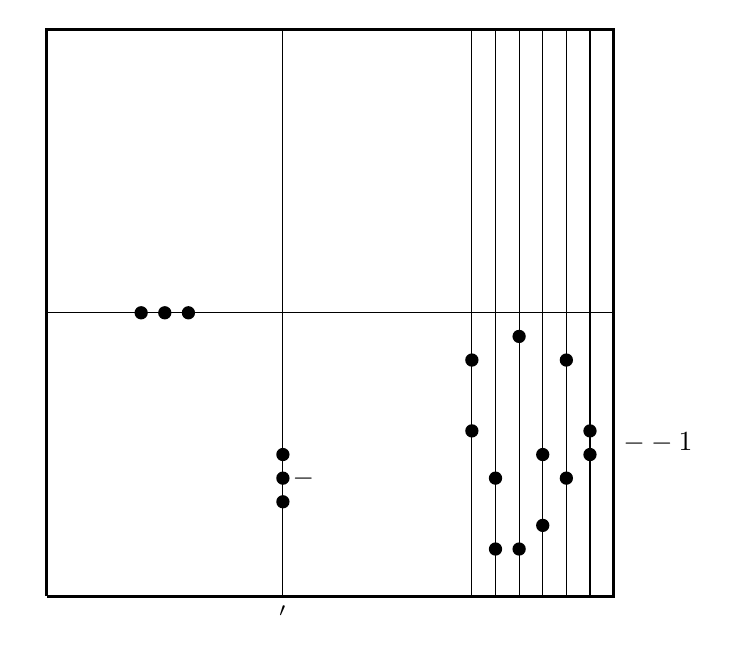
\begin{tikzpicture}[scale=1.2]
    %Draw plane
    \draw[very thick] (0,0) -- (6,0) -- (6,6) -- (0,6) -- (0,0);
    
    %Draw left/middle/right divisions
    %\draw[dotted] (2,0) -- (2,6);
    %\draw[dotted] (4,0) -- (4,6);
    
    % Draw L
    \draw[] (0,3) node[left] {$\Ln$} -- (6,3);
    \fill[black] (1,3) circle (2pt);
    \fill[black] (1.5,3) circle (2pt);
    \fill[black] (1.25,3) node[above] {$\noodle$} circle (2pt);
    
    % Draw \threshold - \noodle line
    \draw[] (2.5,0) -- (2.5,6);
    \fill[black] (2.5,1.25) node[right] {$\threshold - \noodle$} circle (2pt);
    \fill[black] (2.5,1) circle (2pt);
    \fill[black] (2.5,1.5) circle (2pt);
    \draw[] (2.5,0) node[below] {$\Ln'$};
 
    % Draw \threshold - \noodle - 1 lines
    \draw[] (5,0) -- (5,6);
    \fill[black] (5,0.5) circle (2pt);
    \fill[black] (5,2.75) circle (2pt);
    \draw[] (4.75,0) -- (4.75,6);
    \fill[black] (4.75,1.25) circle (2pt);
    \fill[black] (4.75,.5) circle (2pt);
    \draw[] (4.5,0) -- (4.5,6);
    \fill[black] (4.5,1.75) circle (2pt);
    \fill[black] (4.5,2.5) circle (2pt);
    \draw[] (5.75,0) -- (5.75,6);
    \fill[black] (5.75,1.75) circle (2pt);
    \fill[black] (5.75,1.5) circle (2pt);
    \draw[] (5.25,0) -- (5.25,6);
    \fill[black] (5.25,0.75) circle (2pt);
    \fill[black] (5.25,1.5) circle (2pt);
    \draw[] (5.5,0) -- (5.5,6);
    \fill[black] (5.5,1.25) circle (2pt);
    \fill[black] (5.5,2.5) circle (2pt);
    \draw[] (6,1.625) node[right] {$\threshold - \noodle - 1$};
    \draw[] (5.125,0) node[below] {$\threshold$};


  \end{tikzpicture}
  \caption{An instance of the event $F_\Ln$. Here $\threshold=6$, $\noodle=3$. After one step the intersection of lines $\Ln$ and $\Ln'$ becomes open so $\Ln$ has $\noodle+1$ vertices open. At step 2 the $\threshold$ intersections with $\Ln$ and the other $\threshold$ vertical lines become open. At step 3 all of $\Ln$ becomes open. }
  \label{fig:FL}
\end{center}
\end{figure}

We exhibit the role of $F_\Ln$ (see Fig.~\ref{fig:FL}) in the following lemma. 

\begin{lemma} \label{twostep}
If $\Ln$ is a line parallel to the $e_1$ axis and $F_\Ln$ occurs,
then the entire line $\Ln$ is open after three steps.
\end{lemma}
\begin{comment}
\begin{proof}
If $v \in \Ln_m$ 
and the event
$$\I{\Ln_l}{\noodle}\bigcap\I{\Ln_2(v)}{\threshold-\noodle}$$
occurs then $v$ has at least $\threshold$ neighbors initially open and $v$ is open after one step. Then there are at least $\noodle +1$ sites open in $\Ln_l \cup \Ln_m$ after one step. Thus if $F_\Ln$
occurs there are at least $\threshold$ vertices in $\Ln_r$ that are
open after two steps. Thus the entire line $\Ln$ is open after 
three steps.
\end{proof}
\end{comment}

\begin{remark} Computation of 
$P(F_\Ln)$ is facilitated by independence of the three events. 
A more natural definition would not restrict the orientations of the lines, or 
demand that the event happen in the left, middle or right sections thereof, and would increase the probability by a constant factor, independent of $n$.
\end{remark}


%As $\noodle$ decreases, it's more likely that some line $L$ starts with $\noodle$ points open; but as $\noodle$ increases, it's easier for a typical $L$ to intersect $\threshold - \noodle$ other lines with $\threshold - \noodle$ points initially open. It turns out that these balance at 
We set $\noodle =\left\lceil \frac{(d-1)\threshold}{d} \right\rceil -1$ and  $p = n^{-1-\frac{d}{\threshold}}f(n)$, where $f(n)$ is any function such that $f(n) \to \infty$. 
We will show that in this regime some line becomes open asymptotically almost surely.
We will use the following elementary fact about the binomial distribution. 

\begin{lemma} \label{binomlemma}
Assume that $S$ is Binomial$(n,p)$, with large $n$ and $p=p(n)$, and that $k$ does not depend on $n$. 
If $np=O(1)$, then $P(S\ge k)\ge c (np)^k$ for some constant $c$ dependent on $k$. 
If $np\to\infty$, then  $P(S\ge k)\to 1$.
\end{lemma}



\begin{lemma} \label{probA}
Fix $v \in V$ and $ \threshold, d \geq 3$. Let $p=n^{-1-\frac{d}{\threshold}}f(n)$ where $f(n) \to \infty$. Then for any $c>0$, the probability that there exists an $e_1$-parallel line $\Ln$ in $P_{1,2}(v)$ such that $F_\Ln$ occurs
%$$\left( \bigcup_{L} \I{L_l}{\noodle}\right) \bigcap ??$$ 
is at least  $cn^{2-d}$ for $n$ sufficiently large.
%where the union is over $e_1$-parallel lines $L$.
\end{lemma}

%\note{The assumption $\theta\ge d$ seems to be necessary (twice!) in this lemma.}

\begin{proof}
As the event in the statement is increasing, its probability is monotone in $p$. Thus we may 
assume that $f(n)$ grows to $\infty$ as slowly as we need in the proof. 

Note that when $\threshold, d \geq 3$ then $\noodle d/\threshold \geq 1$ as
$$\noodle d/\threshold \geq \left( \frac{(d-1)\threshold}{d} -1\right) \frac{d}{\threshold} = d-1- d/\threshold.$$  
The right hand side is strictly 
greater than 1 except if $d=\threshold=3$. We assume that at least one of $d$ and $\threshold$ 
is at least 4, and leave the exceptional case to the reader. 

The three events that define $F_\Ln$ depend on disjoint sets of sites, so they are independent
and we compute their probabilities separately. 
Furthermore, for the set of lines $\Ln$ we consider, the events 
$\Gone{\Ln}$ and $\Gtwo{\Ln}$ do not depend on $\Ln$, which will thus be dropped from 
the notation.
For any $\Ln$, by Lemma \ref{binomlemma}
\begin{eqnarray*}
\prob(\I{\Ln_l}{\noodle})
 &\geq& c_1  (np)^{\noodle}\\
 &\geq& c_1  (f(n)n^{-d/\threshold})^{\noodle}.
\end{eqnarray*}
As this is $o(1/n)$ we can use Lemma \ref{binomlemma} again to get that
$$\prob\big(\text{$\exists \Ln$ such that $\I{\Ln_l}{\noodle}$ occurs } \big) \geq  c_2  n (f(n)n^{-d/\threshold})^{\noodle}.$$
%
%There are $n$ lines in the union, and they depend on disjoint vertex sets. So we have
%$$\prob\left( \bigcup_{L} \I{L_l}{\noodle}\right) = 1 - \left(1-\prob\left( \I{L_l}{\noodle}\right)\right)^{n^{d-1}}.$$
%For a fixed $L$, we have 
%$$\prob\left( \I{L_l}{\noodle}\right) \ge c (n p)^\noodle = c f(n)^\noodle n^{-d+1}$$
% for some constant $c$. So 
%$$ 1 - \left(1-\prob\left( \I{L_l}{\noodle}\right)\right)^{n^{d-1}} \ge 1 - \left(1 - \frac{cf(n)^\noodle}{n^{d-1}}\right)^{n^{d-1}} \to 1$$
%as long as $f(n)$ does not grow too quickly; since the event
%$$\prob\left( \bigcup_{L} \I{L_l}{\noodle}\right) $$
%is increasing, its probability is monotonic in $p$ and the lemma holds.
%
\begin{comment}
\begin{eqnarray*}
\prob(\I{\Ln_l}{\noodle})
 &\geq&  {n/3 \choose \noodle}p^{\noodle}(1-p)^{n/3-\noodle}\\
 &\geq& c_1  (np)^{\noodle}\\
 &\geq& c_1  (f(n)n^{-d/\threshold})^{\noodle}.
\end{eqnarray*}
Provided that $f(n)$ does not grow too quickly the right hand side is much smaller than $1/n$ so we get
$$\prob\left(\text{$\exists \Ln$ such that $\I{\Ln_l}{\noodle}$ occurs}\right) \geq  .5 c_1  n (f(n)n^{-d/\threshold})^{\noodle}.$$
\end{comment}

To estimate the second probability, observe that 
$$\prob(\I{\Ln_2(v)}{\threshold-\noodle})\ge c_3 (np)^{\theta-r},$$
which is $o(1/n)$, as $r<(d-1)\threshold/d$. Thus 
\begin{eqnarray*}
\prob(\Gonez)
 &\geq& c_4 n (np)^{\threshold- \noodle}\\
 &\geq& c_4 n (f(n)n^{-d/\threshold})^{\threshold- \noodle}.
\end{eqnarray*}

For the third probability, 
$$\prob(\I{\Ln_2(v)}{\threshold-\noodle})\ge c_5 (np)^{\theta-r-1},$$
and 
\begin{eqnarray*}
n\cdot (np)^{\theta-r-1}
 &\geq&   f(n)^{\threshold - \noodle - 1}n^{1-d+(\noodle+1)\frac{d}{\threshold}} \to \infty
\end{eqnarray*}
as $n\to\infty$, 
so Lemma \ref{binomlemma} implies that 
$$
\prob(\Gtwoz) \to 1,
$$
and for large $n$ the probability is bounded below by a constant $c_6>0$.
Multiplying together the probabilities, we have that for any $c$ and all sufficiently large $n$
%the probability that there exists $L$ in $P_{1,2}(v)$ such that that $F_L$ occurs 
%is bounded below by
\begin{eqnarray*}
\lefteqn{\prob(\text{$\exists$ $\Ln$ in $P_{1,2}(v)$ such that that $F_\Ln$ occurs} )}\hspace{1in}&&\\
 &=&\prob(\exists \Ln \text{ such that }\I{\Ln_l}{\noodle})\prob( \Gonez)\prob( \Gtwoz)\\
 &\geq& c_2n(f(n)n^{-d/\threshold})^{\noodle}c_4n (f(n)n^{-d/\threshold})^{\threshold- \noodle}c_6\\
&=& c_7f(n)^\threshold n^{2-d} \\
&>& c n^{2-d},
\end{eqnarray*}
ending the proof.
\begin{comment}
The case when $d=\threshold=3$ is 
almost identical except the roles of the first and second events are reversed. This happens because $\noodle=1<\threshold-\noodle =2$. This is the only choice of $d$ and $\threshold$ for which $\noodle < \threshold -\noodle$. We leave the details to the reader.
\end{comment}
%There are $n^{d-1}$ lines in the union, and they depend on disjoint vertex sets. So we have
%$$\prob\left( \bigcup_{L} \I{L_l}{\noodle}\right) = 1 - \left(1-\prob\left( \I{L_l}{\noodle}\right)\right)^{n^{d-1}}.$$
%For a fixed $L$, we have 
%$$\prob\left( \I{L_l}{\noodle}\right) \ge c (n p)^\noodle = c f(n)^\noodle n^{-d+1}$$
% for some constant $c$. So 
%$$ 1 - \left(1-\prob\left( \I{L_l}{\noodle}\right)\right)^{n^{d-1}} \ge 1 - \left(1 - \frac{cf(n)^\noodle}{n^{d-1}}\right)^{n^{d-1}} \to 1$$
%as long as $f(n)$ does not grow too quickly; since the event
%$$\prob\left( \bigcup_{L} \I{L_l}{\noodle}\right) $$
%is increasing, its probability is monotonic in $p$ and the lemma holds.
\end{proof}

%\begin{lemma}
%\label{crosses}
%Let $p=n^{-1-\frac{d-1}{\noodle}}f(n)$ and suppose $f(n) \to \infty$.
%Then for a given $e_1$-parallel $L$, $$\prob\big(\Gtwo{L}\big) \to 1.$$
%\end{lemma}
%
%\begin{proof}
%The probability that a given cross line $L'$ has at least $\threshold - \noodle$ points initially open is (provided $f(n)$ does not grow too quickly)
%
%\begin{eqnarray}
%\prob(\I{L'}{\threshold-\noodle}) &\ge& {n \choose {\threshold-\noodle}}p^{\threshold-\noodle}(1-p)^{n-\threshold+\noodle} \nonumber\\
%&\geq& k (pn)^{\threshold-\noodle} \nonumber\\
%&\geq& k f(n)^{\threshold - \noodle} n^{-\frac{d-1}{\noodle}(\threshold - \noodle)} \\
%&\geq& k f(n)^{\threshold - \noodle} n^{-1} .
%\label{badgers}
%\end{eqnarray}
%The last exponent of $n$ is at least $-1$. So since the events $\I{L'}{\threshold-\noodle}$ are independent then
%$\sum_{L'} \one_{\I{L'}{\threshold-\noodle}}$
%is a
%$$ \text{Binomial$(n,\prob(\I{L'}{\threshold-\noodle}))$}$$
% random variable.
%By (\ref{badgers}) the means $$n\cdot \prob(\I{L'}{\threshold-\noodle})$$
%of this sequence of random variables go to $\infty$. By the Poisson approximation
%to binomial random variables, since the means are going to infinity the probability that 
%the random variable
%is less than any fixed value goes to 0. 
%Thus the probability that it is at least $\threshold-\noodle$ goes to one.
%\end{proof}
%
\begin{theorem} \label{bicuspid}
Suppose $p = n^{-1-\frac{d}{\threshold}}f(n)$ with $f(n) \to \infty$. Then $\prob(\cup_\Ln F_\Ln)\to 1$ as $n \to \infty$, where the union is taken over all $e_1$-parallel lines. Thus, with probability going to 1, some line becomes open after three steps.
\end{theorem}

\begin{proof}
We can choose $n^{d-2}$ distinct vertices $v_i$ such that $P_{1,2}(v_i)$ are disjoint. Then the
events that there exist $\Ln$ in $P_{1,2}(v_i)$ where $F_\Ln$ occurs are independent.
Moreover, 
$$n^{d-2}\prob(\exists \Ln \text{ in $P_{1,2}(v_i)$ such that $F_\Ln$ occurs})
\geq n^{d-2}cn^{2-d}=c$$
for any fixed $c$. Thus
Thus $\prob(\cup_\Ln F_\Ln)\to 1$ by Lemma \ref{binomlemma}. 
\end{proof}
%\begin{proof}
%Let 
%$$A=\bigcup_{L \parallel e_1} \I{L_l}{\noodle} $$
%and 
%$$B=\bigcup_{L \parallel e_1} \I{L_l}{\noodle} \cap \Gtwo{L}.$$
%Then 
%\begin{eqnarray*}
%%$$
%\prob\left(\bigcup_L{F_L} \right)
%&\ge& \prob(B)=\prob(A\cap B)\\
%&=&\prob(A)\prob(B|A)\\
%&= &\prob(A) \prob(\Gone{L}).
%\end{eqnarray*}
%%$$
%The last equality is true because $\I{L_l}{\noodle}$ and $\Gone{L}$ are independent.
%By Lemmas \ref{probA} and \ref{crosses} the two terms on the right hand side are going to one.
%\end{proof}

%If we ignore the ceiling function in $\noodle = \lceil \frac{d-1}{d}\threshold\rceil$ (or if $\threshold$ is divisible by $d$), the exponent $-1-\frac{d-1}{\noodle} = -1-d/\threshold$. (And note that $-1-\frac{d}{\threshold} = -1-\frac{d-1}{\noodle} + o(\threshold^{-3/2})$.) This is best possible. 
%%Indeed, let 
%%$$E=\{\exists v: \omega_1(v)\neq \omega_0(v)\}$$ be the event that any percolation whatsoever happens.
%Remember that 
%$$\abovethresh=\left\{ \exists v: \sum_{w \sim v}\omega_w\geq \threshold \right\}.$$
\begin{theorem}\label{molar}
Let $p = n^{-1-d/\threshold}f(n)$. If $f(n) \to 0$, then $\prob(\abovethresh) \to 0$. 
%If $f(n) \to \infty$ then $\prob(\abovethresh) \to 1$.
\end{theorem}

\begin{proof} 
Using the union bound, 
\begin{eqnarray*}
\prob(\abovethresh) 
&\leq& \sum_{v \in V}\prob\left(\sum_{w \sim v}\omega_0(w)\geq \threshold \right)\\
&=& n^d\prob\left(\sum_{w \sim v}\omega_0(w)\geq \threshold \right)\\
&\le& n^d{n \choose \threshold}p^\threshold\\
&\le& f(n)^\threshold 
\end{eqnarray*}
which approaches 0 as $n \to \infty$.
%
%Now let $f(n) \to \infty$. {\bf??? Use Chen Stein here if possible.}
\end{proof}
%It's worth noting that if $\threshold = 2$, $d=3$, the true critical exponent for the entire graph to become open is $n^{-2.5} = n^{-1-\frac{d}{\threshold}}$. (To see this note that  two points in one  plane and one point in a different plane are  initially open iff every vertex becomes open). So it may be possible to make the two exponents coincide in general, even if $\threshold$ isn't divisible by $d$.

\begin{pfofthm}{Theorem \ref{la liga}}
Combining Theorems \ref{bicuspid} and \ref{molar} proves the result. 
\end{pfofthm}

%In conclusion, we remark that the assumption $\threshold\ge 3$ is needed to make $\noodle \ge 1$.

\section{Open two-dimensional subgraphs} \label{nessforplanes}
In previous sections we have encountered several possibilities
for a vertex $v$ to become open:
\begin{itemize}
\item $v$ is initially open;
\item the neighborhood of $v$ has at least $\threshold$ vertices initially open, causing $v$ to become open by time 1; and 
\item a line containing $v$ has at least $\threshold(d-1)/d$ vertices initially open, 
with some additional open sites ``nearby'' (see Section 
\ref{lines}).
\end{itemize}

Let $\D$ be the event that some plane eventually becomes open.
In this section we show that if $p$ is sufficiently small then with high probability all of the vertices that are eventually open satisfy a condition like one of the three above.
By doing this we prove an upper bound on the 
probability of $\D$ and consequently a lower bound on the threshold probability $p_c(2,d)$.  
%We do this by 
%defining conditions, in the form of event $E$ below, that enumerate the asymptotically necessary conditions for a vertex to 
%vertex to become open. The motivation for this is the idea that if a vertex $v$ eventually becomes open,
%then it's likely that either one of the lines through $v$ started with many points on, or that the neighborhood of $v$ started with
%almost $\threshold$ points on.


Let $A$ be some integer, $1\leq A\leq \threshold$, which we will specify later. Let $E$ be the event that there exists a vertex $v$ such that:
\begin{enumerate}
\item $v$ is initially not open; \label{aretha}
\item the neighborhood of $v$ has at most $A$ vertices initially open; \label{thebigo}
\item each line containing $v$ has at most $A/2$ vertices initially open; and \label{wilsonpickett}
\item $v$ becomes open. \label{samcooke}
\end{enumerate}
Our strategy to demonstrate that $\prob(\D)$ is small for sufficiently small $p$ is to  
show that  $\prob(E)$ and $\prob(\D \setminus E)$ are both small.

For each vertex $v$, let $E_v$ be the event that $v$ satisfies (1)--(4), and none among
such vertices becomes open earlier. If the event $E$ occurs then there must be 
a first time a vertex satisfying (1)--(4) exists, thus $E \subseteq \cup_v E_v$, and
consequently, $\prob(E) \le n^d \prob(E_v)$.

\begin{lemma}\label{cajunsprel1}
Suppose $p = o(n^{-1-\beta})$ with $\beta > (\frac{2d^2}{\threshold-A}+1)\frac{2}{A}$.  Fix a line $\Ln$. The probability that $\Ln$ contains at least $\frac{\threshold-A}{2d}$ vertices $v$ 
that have at least $A/2$ initially open points in $\mathcal{N}(v)\setminus \Ln$  is 
$$%\hbox{const } \cdot 
o\left(n^{\frac{\threshold-A}{2d}(1-\beta\frac{A}{2})}\right).
$$
\end{lemma}
\begin{proof}
The reduced neighborhoods $\mathcal{N}(v)\setminus \Ln$, $v\in\Ln$, are pairwise 
disjoint, and in each
the number of initially open vertices is a Binomial$((d-1)(n-1),p)$ random variable.
The probability that such a random variable is at least $A/2$ is bounded 
by a constant times $(np)^{A/2}=o\left(n^{-\beta A/2}\right)$. These
random variables are independent, thus the probability that at least $\frac{\threshold-A}{2d}$ of them
are at least $A/2$ is  $o\left((n\cdot n^{-\beta A/2})^\frac{\threshold-A}{2d}\right)$.
\end{proof}

\begin{lemma}\label{cajunsprel2}
Assume $p$ satisfies the same bound as in Lemma \ref{cajunsprel1}. 
Fix a line $\Ln$. The probability that $\Ln$ has at least $\frac{\threshold-A}{2d}$ vertices $w$,
for which there exists a line $\Ln'\ne \Ln$ through $w$ such that 
$\Ln'\setminus \{w\}$ contains at least $A/2$ initially open points is 
$$o\left(n^{\frac{\threshold-A}{2d}(1-\beta\frac{A}{2})}\right).$$
\end{lemma}
\begin{proof} We need to bound the probability of at least  
$\frac{\threshold-A}{2d}$ successes in 
$n(d-1)$ independent trials, each of which is a success with  
the probability that a given line has at least $A/2$ points initially open. 
Same estimates as in the proof of Lemma \ref{cajunsprel1} apply.
\end{proof}


\begin{lemma} \label{cajuns}
Assume $p$ satisfies the same bound as in Lemma \ref{cajunsprel1}.
Then $\prob(E) \to 0$ as $n \to \infty$.
\end{lemma}
\begin{proof}
As we have already observed, $\prob(E) \le n^d\prob(E_v)$. Now, if $E_v$ occurs, by (\ref{thebigo}) at least $\threshold-A$ vertices in the neighborhood of $v$ must be initially closed but become open strictly before $v$; therefore, they violate at least one of (1)--(4). But since they are not 
open initially and become open, they must violate one of (\ref{thebigo}) or (\ref{wilsonpickett}). By the pigeonhole principle, of the $d$ lines through $v$, at least one must either contain $\frac{\threshold-A}{2d}$ vertices which violate (\ref{thebigo}), or $\frac{\threshold-A}{2d}$ vertices which violate (\ref{wilsonpickett}).

By Lemmas \ref{cajunsprel1}  and \ref{cajunsprel2}, each of these happens with probability 
$$ o\left(  n^{\frac{\threshold-A}{2d}(1-\beta\frac{A}{2})}\right).$$
Rearranging using the inequality $\beta > (\frac{2d^2}{\threshold-A}+1)\frac{2}{A}$, we see that 
$\prob(E_v)=o(n^{-d})$, as claimed.
\end{proof}
 
\begin{lemma} \label{activenotE}
Let $p = n^{-1-\beta}$, with $\beta > 0$, and assume $A\ge 4$. 
Then $\prob(\D \setminus E) \to 0$ as $n \to \infty$.
\end{lemma}
\begin{proof}
There are ${d \choose 2}n^{d-2}$ planes, $\plane$, and
$\D = \cup_\plane \{\hbox{$\plane$ becomes open}\}$,
so we have
$$\prob(\D \setminus E) \le {d \choose 2}n^{d-2} \prob(\{{\plane}\text{ becomes open}\}\setminus E).$$

Now if $\plane$ becomes open but $E$ does not occur, then since each point in $\plane$ becomes open, they must all violate one of (\ref{aretha}), (\ref{thebigo}), or (\ref{wilsonpickett}). By the pigeonhole principle, at least $n^2/3$ of these points must together violate a single condition. We will check that the probabilities of these three cases are $o(n^{-(d-2)})$. In fact, we will see
that they are exponentially small by reducing each case to a large deviation probability 
involving a Binomial random variable with a small chance of success. We will use
the fact that neighborhoods of two points in $\plane$ do not intersect outside $\plane$. 

\begin{itemize}
\item $\prob(n^2/3$ vertices in $\plane$ are initially open$)$ is exponentially small 
in $n^2$, as $p=o(1)$.  
%The probability of this is bounded by 
%$${{n^2} \choose {n^2/3}}p^{n^2/3} \le  2^{n^2}(p^{1/3})^{n^2} =o\left(n^{d-2}\right).$$

\item $\prob(n^2/3$ vertices in $\plane$ are each on a line with $A/2$ points initially open$)$
is exponentially small in $n$. 

As every line covers at most $n$ points in $\plane$, this event implies that there 
are at least $n/(3d)$ parallel lines, in some direction $e_i$,  
each with at least $A/2$ points initially open.  
The probability that a given line has at least $A/2$ points initially 
open is $O((np)^{\lfloor A/2\rfloor})=o(1)$, thus the probability that $n/(3d)$ lines in a given direction 
$e_i$ satisfy this is exponentially small in $n$.

\begin{comment}
 The probability of this is at most
$$2{n \choose n/6}\left({n \choose A/2}p^{A/2}\right)^{n/6}\leq 
2\cdot 2^n\left(n^{-\beta A/2}\right)^{n/6}\leq 2\cdot 2^n n^{-n/6}
=o\left(n^{-(d-2)}\right) .$$
\end{comment}

\item  $\prob(n^2/3$ vertices in $\plane$ each have at least $A$ initially open vertices 
in their neighborhoods$)$ is exponentially small in $n$. 

If a vertex $w$ has at least $A$ initially open vertices in its neighborhood  
then either one of the two lines through $w$ in $\plane$ contain at least $A/4$  
initially open vertices or the $d-2$ lines through $w$ not in $\plane$ together  
contain at least $A/2$ initially open vertices.
This implies that either (a) there are at least $n/12$ parallel lines in $\plane$ with at least $A/4$ vertices initially open, or (b) there are at least $n^2/6$ vertices with at 
least $A/2$ vertices in their neighborhoods outside of 
$\plane$.  

The probability of (a) is exponentially small by the same argument as in the previous case. 
For a fixed $w$, the probability that $(d-2)(n-1)$ sites in $\mathcal{N}(w)\setminus \plane$ 
contain at least $A/2$ initially open sites 
is again $O(np)=o(1)$. Thus the probability of (b) is exponentially small in $n^2$. 

\begin{comment}
The probability of the first is at most
$$2{n \choose n/12}\left({n \choose A/4}p^{A/4}\right)^{n/12}\leq 
2\cdot 2^n\left(n^{-\beta A/4}\right)^{n/12}\leq n^{-cn}=o\left(n^{-(d-2)}\right)$$
and the second has probability at most
$$ {n^2 \choose n^2/6}\left({dn \choose A/2}p^{A/2}\right)^{n^2/6}\leq 
c \cdot 2^{n^2}\left(n^{-\beta A/2}\right)^{n^2/6}\leq n^{-cn^2}=o\left(n^{-(d-2)}\right).$$
\end{comment}
\end{itemize}
Therefore,  $\prob(\D \setminus E)$ goes to 0 exponentially fast.
\end{proof}

\begin{pfofthm}{Theorem \ref{epl}} To get the lower bound
set $A=\lfloor \threshold -\sqrt{\threshold}\rfloor$. Then Lemmas \ref{cajunsprel1}--\ref{cajuns}
are (for large enough $\theta$) satisfied with
$$\beta = \frac{2}{\threshold} + \frac{4d^2 + 3}{\threshold^{3/2}}.$$
The upper bound was proved in Theorem \ref{2d-largetheta-upper-thm}. 
\end{pfofthm}

\section{Further questions and conjectures}
\label{open}

We begin with a general form of threshold probabilities; we believe that the answer to the question 
below is positive.

\begin{question} Do there exist positive constants  $c_1=c_1(i,d)$ and $c_{3/2}=c_{3/2}(i,d)$, so that, for
all $i$ and $d$, a lower bound and an upper bound for $p_c(i,d)$ are both  of the form 
$$n^{-1 - \frac{c_1}{\threshold} - \frac{c_{3/2}}{\threshold^{3/2}}+o(\threshold^{-3/2})},$$
for large enough $n$?
\end{question}

We next ask whether it is possible that generation of open planes  
does not likely lead to spanning of the entire graph when $d\geq 4$.

\begin{question}
Can one find $d$ and $\theta>2$ such that $\log_n(p_c(2,d))-\log_n(p_c(d,d))$ is bounded away from 0 as $n \to \infty$, i.e. $p_c(2,d)\approx n^{-\zeta}$ and $p_c(d,d)\approx n^{-\xi}$
with $\zeta>\xi$? Does this hold for all $\theta$ and $d \geq 4$? Note that it does not hold for $d=3$ by (\ref{cloudforestcafe}).
\end{question}

It would be desirable to have a general method to determine the critical exponent for any given 
(small) $d$ and $\threshold$;
here we merely recall the simplest unsolved instances. 


\begin{question}
When $d=3$, we know the critical exponents for $\theta = 2,3,4,5,6,7,9,11$;  
what are the correct exponents for $\theta = 8, 10$ and $\theta \geq 12$?
\end{question}

%%%%%%%%% Appendix
%\appendix % Not appendix in the thesis
\section{Poisson convergence for $d=\threshold=3$}
\label{ap:poisson}
In this section we outline the proof of Lemma~\ref{3d-poisson-lem} regarding Poisson convergence of the random variables that count the configurations that lead to spanning when $d=\threshold=3$ and $p = an^{-2}$.  Our approach is to apply the Chen-Stein method~\cite{poissonbook}, and to do so we need to introduce some notation.

We want to show that a collection of random variables, which are sums of indicator random variables, converge to independent Poisson random variables in the limit.  That is, suppose we have disjoint sets of indices, $\Gamma_1, \Gamma_2, \ldots, \Gamma_\ell$, let $\Gamma = \cup_{i=1}^\ell \Gamma_i$, and for each $\gamma \in \Gamma$ suppose $I_\gamma$ is an indicator random variable.  For $i=1, \ldots, \ell$ let $W_i = \sum_{\gamma\in \Gamma_i} I_\gamma$ and suppose that $EW_i = \lambda_i$ and $EI_\gamma = p_\gamma$.  In our application, the index sets are going to be $V$ for the indicators of the basic and enhanced basic events, and $\lineset$ for the indicators of the line, $\emptyset$-line, enhanced line, and non-enhanced line events.

To apply the Chen-Stein method in many cases we need to construct a coupling for every fixed $\gamma \in \Gamma$ between $I_\eta$ and $J_{\eta\gamma}$ so that
\begin{align}
\label{coupling}
(J_{\eta\gamma})_{\eta\neq \gamma} \deq (I_\eta | I_\gamma=1)_{\eta\neq\gamma}.
\end{align}
Many of the indicators that we have constructed are increasing functions of $\omega_0$, which makes those sets of indicators positively related (\cite{poissonbook}, Section 2.1).  However, the $\emptyset$-line and non-enhanced line indicators, $\OL_\Ln$ and $\NEL_\Ln$, are not increasing functions of $\omega_0$, so whenever these appear we are unable to use the simpler form of the Poisson convergence theorem.  Instead, we will explicitly define the couplings below, and use Theorem 10.J of \cite{poissonbook}, which we state below as Lemma~\ref{chen-stein}.

Suppose $X$ and $Y$ are two $\mathbb{Z}^m$-valued random variables with laws $\mu_X$ and $\mu_Y$, and recall that the total variation distance between $\mu_X$ and $\mu_Y$ (or with an abuse of notation, between $X$ and $Y$ or $X$ and $\mu_Y$) is
\begin{align*}
d_{TV}(X,Y) = d_{TV}(\mu_X,\mu_Y) := \sup_{A\subset \mathbb{Z}^m} \abs{\mu_X(A) - \mu_Y(A)} = \frac{1}{2} \sum_{k \in \mathbb{Z}^m} \abs{\mu_X(k) - \mu_Y(k)} .
\end{align*}
Let $P_\lambda$ denote the law of a Poisson($\lambda$) random variable (taking values in $\mathbb{Z}_{+}$).  The Chen-Stein method gives us the following bound on the total variation distance between the joint law of $(W_1, W_2, \ldots, W_m)$ and $\prod_{i=1}^m P_{\lambda_i}$.
\begin{lemma}
\label{chen-stein}(\cite{poissonbook}, Theorem 10.J and Corollary 10.J.1)
If $W_i$ are defined as above with $\lambda_i = EW_i$ for $i=1, \ldots,\ell$, with $EI_\gamma = p_\gamma$, then
\begin{align}
\label{cs1}
d_{TV}\left((W_1, \ldots, W_m), \ \prod_{i=1}^m P_{\lambda_i}\right) \leq \sum_{\gamma \in \Gamma} p_\gamma^2 + \sum_{\substack{\gamma, \eta \in\Gamma \\ \gamma\neq\eta}} p_\gamma \E\abs{J_{\eta\gamma} - I_\eta}.
\end{align}
If $\{I_\gamma\}_{\gamma\in\Gamma}$ are positively related then
\begin{align}
\label{cs2}
d_{TV}\left((W_1, \ldots, W_m), \ \prod_{i=1}^m P_{\lambda_i}\right) \leq \sum_{\gamma \in \Gamma} p_\gamma^2 + \sum_{\substack{\gamma, \eta \in\Gamma \\ \gamma\neq\eta}} \Cov(I_\gamma, I_\eta).
\end{align}
\end{lemma}
\begin{remark}
In all of our applications of Lemma~\ref{chen-stein}, the first sum on the right hand side is easy to control, since it merely requires that $p_\gamma$ are uniformly small.  In the case of events indexed by $\lineset$ this sum is $O(n^{-2})$, since there are $O(n^2)$ summands and the probability of a line configuration is $O(n^2p^2) = O(n^{-2})$.  Similarly, in the case of basic or enhanced basic events this sum is $O(n^{-3})$.  The important part of the right hand side is the term $\E\abs{J_{\eta\gamma} - I_\eta} = \prob{(J_{\eta\gamma} \neq I_\eta)}{}$, which requires bounding the probability that our coupling destroys or creates the event indicated by $I_\eta$.  In the case of positively related indicators, no explicit coupling is needed, and we must merely bound the covariances between the relevant indicators.
\end{remark}


%%%% Construction of coupling
\subsection*{Construction of couplings}
Observe that in equation (\ref{goodevent}), the last term involves random variables that are sums of indicators that are not positively related.  So, for each of the indicators $\B_{\vect{v}}, \OL_\Ln, \EL_{\Ln}, \NEL_{\Ln}$ and every $\vect{v}\in V$ and $\Ln \in \lineset$, we must construct a suitable coupling between all of the remaining indicators and their conditioned versions as in (\ref{coupling}).  As in (\ref{coupling}), we will use the letter $J$ for coupled indicator random variables.

Once we show that these random variables appearing in the last term of~(\ref{goodevent}) converge jointly to independent Poissons, we will be able to compute the limiting probabilities for all of the terms except the second, which involves the $\ebasic$ and $\lin$ random variables.  We will treat this term separately using the simpler form of Lemma~\ref{chen-stein}, since the enhanced basic and line indicators are positively related.

Our goal is to show that the second summation in~(\ref{cs1}) is $O(n^{-1})$ under the couplings that we construct.  We will need to construct four couplings, one for each type of indicator, and for each coupling we have four comparisons (to each of the four types of indicators) that need to be made.  Furthermore, for each comparison, there are several cases that need to be checked depending on the relative positions of the vertices and lines that index each event.  There are many cases that need to be verified, but the arguments quickly become repetitive, thus we merely outline the proof and give complete details in two typical cases (see proofs of Lemmas~\ref{nel-coupling-lem} and~\ref{ebasic-line-lem}).

We begin with the simplest case, the {\em basic coupling} for conditioning on $\B_{\vect{v}} = 1$ for a fixed $\vect{v}\in V$.  In this case, we merely need each of the three lines containing $\vect{v}$ to contain at least one open vertex.  To achieve this, we extend the probability space by possibly resampling the vertices in each of the three lines until this condition is met.  That is, if a line through $\vect{v}$ already contains an open vertex, nothing is resampled for that line, and the original configuration is kept, otherwise it is repeatedly replaced with an independent configuration until it does contain an open vertex.  Also, it is important to note that none of the other vertices in the initial configuration, $\omega_0$, are altered.  Then, $\JB_{\vect{wv}}, \JOL_{\Ln\vect{v}}, \JEL_{\Ln\vect{v}}, \JNEL_{\Ln\vect{v}}$ are the indicator random variables of the corresponding events after the local resampling is completed.  Since $\vect{v}$ is fixed and the Hamming torus is transitive, we will drop the index $\vect{v}$ in the conditioning on $\B_{\vect{v}}=1$.  % Also, we work with the indicators $\Lfoo_{\Ln}$ and $\JL_{\Ln}$ when convenient, since $\NEL_\Ln = \Lfoo_{\Ln} - \EL_\Ln$.
\begin{lemma}
\label{basic-coupling-lem}
Under the basic coupling, the following sums are all $O(n^{-1})$
\begin{align*}
\sum_{\vect{v}\in V} \sum_{\substack{\vect{w}\in V \\ \vect{w}\neq\vect{v}}} E\B_{\vect{v}}\ \prob{\left(\B_{\vect{w}} \neq \JB_{\vect{w}}\right)}, & \hspace{1cm} \sum_{\vect{v}\in V} \sum_{\Ln \in \lineset} E\B_{\vect{v}}\ \prob{\left(\OL_\Ln \neq \JOL_\Ln\right)},
\hspace{1cm}  \\
\sum_{\vect{v}\in V} \sum_{\Ln \in \lineset} E\B_{\vect{v}}\ \prob{\left(\NEL_\Ln \neq \JNEL_\Ln\right)}, &\hspace{1cm} \sum_{\vect{v}\in V} \sum_{\Ln \in \lineset} E\B_{\vect{v}}\ \prob{\left(\EL_\Ln \neq \JEL_\Ln\right)}.
\end{align*}
\end{lemma}
The next simplest coupling is the {\em $\emptyset$-line coupling} for the conditioning on $\OL_\Ln = 1$ for a fixed $\Ln \in \lineset$.  For this coupling, we need the line $\Ln$ to contain at least two initially open vertices, so we first resample the vertices in $\Ln$ if necessary until this condition is met.  Given the locations of the open vertices in $\Ln$, we need the two planes containing $\Ln$ to have no open vertices that are not neighbors of the open vertices in $\Ln$.  To achieve this, we simply remove any violating vertices from~$\omega_0$.  In the next three lemmas, we
use indicators $J$, with proper subscripts and superscripts, in an analogous fashion as in Lemma~\ref{basic-coupling-lem}.
\begin{lemma}
\label{ol-coupling-lem}
Under the $\emptyset$-line coupling the following sums are $O(n^{-1})$
\begin{align*}
\sum_{\Ln \in \lineset} \sum_{\vect{w}\in V} E\OL_\Ln\ \prob{\left(\B_{\vect{w}} \neq \JB_{\vect{w}}\right)}, & \hspace{1cm} 
\sum_{\Ln \in \lineset} \sum_{\substack{\Ln' \in \lineset\\ \Ln'\neq \Ln}} E\OL_\Ln\ \prob{\left(\OL_{\Ln'} \neq \JOL_{\Ln'}\right)},
\hspace{1cm}  \\
\sum_{\Ln \in \lineset} \sum_{\Ln' \in \lineset} E\OL_\Ln\ \prob{\left(\NEL_{\Ln'}\neq \JNEL_{\Ln'}\right)}, &\hspace{1cm} 
\sum_{\Ln \in \lineset} \sum_{\Ln' \in \lineset} E\OL_\Ln\ \prob{\left(\EL_{\Ln'} \neq \JEL_{\Ln'}\right)} .
\end{align*}
\end{lemma}

Next, we construct the {\em enhanced line coupling} for the conditioning on $\EL_\Ln = 1$ for a fixed $\Ln \in \lineset$.  To achieve this, we will need the line $\Ln$ to contain at least two open vertices, so we first resample the vertices in $\Ln$ if necessary until this condition is met.  Next, given the locations of the open vertices in $\Ln$, we need that at least one of the two planes containing $\Ln$ has at least one open vertex that is not collinear with an open vertex in $\Ln$.  Again, if necessary, we resample these two planes (excepting the vertices in $\Ln$) simultaneously until this condition is satisfied.  At this point, if one of the two planes containing $\Ln$ has at least  two non-neighboring open vertices, then the coupling is completed.  Otherwise, conditional on the location of the open vertex (or vertices) in $\mathcal{N}(\Ln)$, we need there to be at least one open vertex in the same plane as this vertex (or vertices) but not in the same line.  If one does not exist, then we resample the two (or four) planes containing the open vertex (or vertices) in $\mathcal{N}(\Ln)$ but not containing $\Ln$ until there is at least one open vertex in any of these planes (we do not resample the vertices in $\Ln$, $\mathcal{N}(\Ln)$, or the neighborhood of the open vertices in $\mathcal{N}(\Ln)$).

\begin{lemma}
\label{el-coupling-lem}
Under the enhanced line coupling the following sums are $O(n^{-1})$
\begin{align*}
\sum_{\Ln \in \lineset} \sum_{\vect{w}\in V} E\EL_\Ln\ \prob{\left(\B_{\vect{w}} \neq \JB_{\vect{w}}\right)}, & \hspace{1cm} 
\sum_{\Ln \in \lineset} \sum_{\Ln' \in \lineset} E\EL_\Ln\ \prob{\left(\OL_{\Ln'} \neq \JOL_{\Ln'}\right)},
\hspace{1cm}  \\
\sum_{\Ln \in \lineset} \sum_{\Ln' \in \lineset} E\EL_\Ln\ \prob{\left(\NEL_{\Ln'}\neq \JNEL_{\Ln'}\right)}, &\hspace{1cm} 
\sum_{\Ln \in \lineset} \sum_{\substack{\Ln' \in \lineset\\ \Ln'\neq \Ln}} E\EL_\Ln\ \prob{\left(\EL_{\Ln'} \neq \JEL_{\Ln'}\right)} .
\end{align*}
\end{lemma}

Finally, we construct the {\em non-enhanced line coupling} for the conditioning on $\NEL_\Ln = 1$ for a fixed $\Ln \in \lineset$.  To achieve this, we will need the line $\Ln$ to contain at least two open vertices.  So first we resample the vertices in $\Ln$ if necessary until this condition is met.  Next, given the locations of the open vertices in $\Ln$, we need: 1) that at least one of the two planes containing $\Ln$ has at least one open vertex that is not collinear with an open vertex in $\Ln$, and 2) that neither plane containing $\Ln$ has more than one non-collinear open vertex.  Again, if necessary, we resample these two planes simultaneously until these conditions are met (here we do not resample $\Ln$).  Now, conditional on the locations of the open points in $\mathcal{N}(\Ln)$, we must guarantee that there are no other points outside of $\Ln$ that are coplanar but not collinear with these points.  For this part of the coupling, we simply remove any violating points from $\omega_0$.

\begin{lemma}
\label{nel-coupling-lem}
Under the non-enhanced line coupling the following sums are $O(n^{-1})$
\begin{align*}
\sum_{\Ln \in \lineset} \sum_{\vect{w}\in V} E\NEL_\Ln\ \prob{\left(\B_{\vect{w}} \neq \JB_{\vect{w}}\right)}, & \hspace{1cm} 
\sum_{\Ln \in \lineset} \sum_{\Ln' \in \lineset} E\NEL_\Ln\ \prob{\left(\OL_{\Ln'} \neq \JOL_{\Ln'}\right)},
\hspace{1cm}  \\
\sum_{\Ln \in \lineset} \sum_{\substack{\Ln' \in \lineset\\ \Ln'\neq \Ln}} E\NEL_\Ln\ \prob{\left(\NEL_{\Ln'}\neq \JNEL_{\Ln'}\right)}, &\hspace{1cm} 
\sum_{\Ln \in \lineset} \sum_{\Ln' \in \lineset} E\NEL_\Ln\ \prob{\left(\EL_{\Ln'} \neq \JEL_{\Ln'}\right)} .
\end{align*}
\end{lemma}
\begin{proof}
We now outline the proof by bounding the first summation above.  There are three cases.

\noindent {\em Case 1:} $\vect{w}\in \Ln$.  This term appears in the sum $O(n^3)$ times, and $E\NEL_\Ln = O(n^{-2})$, so we must show that $\prob{(\B_{\vect{w}} \neq \JB_{\vect{w}})} = O(n^{-2})$.  Now there are two subcases, {\em destruction} and {\em creation} respectively: $\prob{(\B_{\vect{w}} = 1, \JB_{\vect{w}} = 0)}$ and $\prob{(\B_{\vect{w}} = 0, \JB_{\vect{w}} = 1)}$.  Clearly, $\prob{(\B_{\vect{w}} = 1, \JB_{\vect{w}} = 0)}\leq \prob{(\B_{\vect{w}} = 1)} = O(n^{-3})$.  Next, in order for the creation event to occur, the resampling procedure must have generated at least one open vertex in both planes containing $\Ln$, and both of these points must lie in the neighborhood of $\vect{w}$.  The probability of this is $O(n^{-2})$, since we require an open vertex in each of two fixed lines.

\noindent {\em Case 2:} $\vect{w} \in \mathcal{N}(\Ln)$.  This term appears in the sum $O(n^4)$ times, and $E\NEL_\Ln = O(n^{-2})$, so we must show that $\prob{(\B_{\vect{w}} \neq \JB_{\vect{w}})} = O(n^{-3})$.  Once again, there are two subcases as above.  The creation event cannot occur in this case because an open vertex in $\mathcal{N}(\Ln)$ that is collinear with $\vect{w}$ must not see any coplanar open vertices (off of $\Ln$), which includes a line in the neighborhood of $\vect{w}$, so $\vect{w}$ can no longer see an open vertex in each direction.  The probability of the destruction event can be trivially bounded by $O(n^{-3})$ as in Case 1.

\noindent {\em Case 3:} $\vect{w} \notin \mathcal{N}(\Ln) \cup \Ln$.  This term appears in the sum $O(n^5)$ times, and $E\NEL_\Ln = O(n^{-2})$, so we must show that $\prob{(\B_{\vect{w}} \neq \JB_{\vect{w}})} = O(n^{-4})$.  Once again, the creation event cannot occur for the same reason as cited in Case 2.  The destruction event can only occur if one of the initially open points in the neighborhood of $\vect{w}$ is in one of the resampled planes.  At most six planes are affected with probability $1-O(n^{-1})$, and with the same probability none of the resampled planes contain a line in the neighborhood of $\vect{w}$.  The probability of the destruction event is at most $O(n^{-4})$, since $\vect{w}$ must first have three open neighbors initially (an event with probability $O(n^{-3})$), and at least one must coincide with one of the resampled planes (an event with probability $O(n^{-1})$).  
\end{proof}

%%%% Pos related case
\subsection*{Positively related case}
Since $\{\EB_{\vect{v}}\}_{\vect{v}\in V}$ and $\{\Lfoo_{\Ln}\}_{\Ln\in \lineset}$ are all increasing functions of $\omega_0$, these collections of indicators are positively related so we may apply the simpler form of Lemma~\ref{chen-stein} by bounding the covariances.
\begin{lemma} 
\label{ebasic-line-lem}
The collections of indicators $\{\EB_{\vect{v}}\}_{\vect{v}\in V}$ and $\{\Lfoo_{\Ln}\}_{\Ln\in \lineset}$ are positively related and the following sums are $O(n^{-1})$
\begin{align*}
\sum_{\vect{v}\in V} \sum_{\substack{\vect{w}\in V\\ \vect{w}\neq \vect{v}}} \Cov(\EB_{\vect{v}},\EB_{\vect{w}}),
 \hspace{1cm} \sum_{\vect{v}\in V} \sum_{\Ln\in\lineset} \Cov(\EB_{\vect{v}},\Lfoo_{\Ln}),
  \hspace{1cm} \sum_{\Ln\in\lineset} \sum_{\substack{\Ln'\in\lineset\\ \Ln'\neq\Ln}} \Cov(\Lfoo_{\Ln},\Lfoo_{\Ln'}).
\end{align*}
\end{lemma}
Note that the bound on the last sum, which involves only indicators of line events, is implied by combining the results for the enhanced line and non-enhanced line couplings in Lemmas~\ref{el-coupling-lem} and~\ref{nel-coupling-lem} by writing $\Lfoo_\Ln = \EL_\Ln + \NEL_\Ln$.
\begin{proof}
We will explain the proof of the bound on the first sum, as the second sum is evaluated in a similar fashion and the third is implied by previous lemmas.  We break up the sum into three cases depending on the Hamming distance between $\vect{v}$ and $\vect{w}$.

\noindent {\em Case 1:} $d(\vect{v},\vect{w})=1$.  There are $O(n^4)$ such terms in the sum, so we need to show that the covariance is $O(n^{-5})$.  In this case it suffices to use the trivial bound $\Cov(\EB_{\vect{v}},\EB_{\vect{w}}) \leq \E\EB_{\vect{v}}\EB_{\vect{w}} = \prob(\event_v^{EB}\cap \event_w^{EB})$, which is the probability that an enhanced basic configuration appears at $\vect{v}$ and at $\vect{w}$.  For this event to occur, $\vect{v}$ must have one open neighbor in each direction, one of which is shared with $\vect{w}$, so $\vect{w}$ needs only one open neighbor in each direction orthogonal to $\vect{w}-\vect{v}$.  This is a total of at least five open points on five fixed lines, which has probability $O((np)^5) = O(n^{-5})$ as desired.

\noindent {\em Case 2:} $d(\vect{v},\vect{w}) =2$.  There are $O(n^{5})$ such terms in the sum, so we need to show that the covariance is $O(n^{-6})$.  Again, it suffices to use the bound $\Cov(\EB_{\vect{v}},\EB_{\vect{w}}) \leq \E\EB_{\vect{v}}\EB_{\vect{w}}$.  In this case, the vertices $\vect{v}$ and $\vect{w}$ have exactly two common neighbors, so there are three cases: zero, one, or two of these common neighbors are initially open.  If neither common neighbor is initially open, then $\vect{v}$ and $\vect{w}$ each independently need one open neighbor in each direction -- a total of six open vertices in six fixed lines, which has probability $O(n^{-6})$.  If one of the common neighbors is open, an event with probability $O(p) = O(n^{-2})$, then $\vect{v}$ and $\vect{w}$ each need an open neighbor in two other directions -- a total of four open vertices in four fixed lines which has probability $O(n^{-4})$.  This gives a probability of $O(n^{-6})$ to the case where one common neighbor is open.  The event that both common neighbors are open has probability $p^2 = O(n^{-4})$, and $\vect{v}$ and $\vect{w}$ each require one more occupied neighbor in one direction, which has probability $O(n^{-2})$ for a total probability of $O(n^{-6})$.

\noindent {\em Case 3:} $d(\vect{v},\vect{w})=3$.  There are $O(n^{6})$ such terms in the sum, so we need to show that the covariance is $O(n^{-7})$, and the trivial upper bound on the covariance will not suffice.  Observe that the planes containing $\vect{v}$ and the planes containing $\vect{w}$ intersect only along 6 lines, and conditional on the event that none of the points on these lines are initially open, $\EB_{\vect{v}}$ and $\EB_{\vect{w}}$ are independent.  Call this event $E_{\text{empty}}$, then since $\EB_{\vect{v}}$ and $\EB_{\vect{w}}$ are increasing functions of $\omega_0$, the covariance is bounded by
\begin{align*}
\Cov(\EB_{\vect{v}},\EB_{\vect{w}}) \leq \prob{(\EB_{\vect{v}}\EB_{\vect{w}} = 1, E_{\text{empty}}^c)}
\end{align*}
We now divide the event $E_{\text{empty}}^c$ into subcases according to which vertices in the intersection are open.  There are two types of vertices in the intersection -- those which are neighbors to either $\vect{v}$ or $\vect{w}$, and those which are only in the same plane as each vertex.  There are exactly 6 vertices in the former category and $6(n-2)$ in the latter.  The probability that $j$ of the 6 vertices in $[\mathcal{N}(\vect{v})\cap\mathcal{N}(\mathcal{N}(\vect{w}))] \cup [\mathcal{N}(\vect{w})\cap\mathcal{N}(\mathcal{N}(\vect{v}))]$ are initially open is $O(p^j) = O(n^{-2j})$.  Conditional on this, $\vect{v}$ and $\vect{w}$ collectively require an initially open vertex in each of the remaining $6-j$ lines in their neighborhoods, which has probability $O(n^{-6+j})$, giving a total probability of $O(n^{-6-j})$ to the event that there are $j$ of these 6 vertices initially open and both enhanced basic events occur.  Therefore, if $j\geq 1$ we are done, otherwise we must consider the case where $j=0$ and then $E_{\text{empty}}^c$
requires that at least one vertex among the $6(n-2)$ vertices in $\mathcal{N}(\mathcal{N}(\vect{v}))\cap\mathcal{N}(\mathcal{N}(\vect{w}))$ are initially open.  This event has probability $O(np) = O(n^{-1})$, and when $j=0$, $\vect{v}$ and $\vect{w}$ still need one open vertex in each line of their neighborhoods, which has probability $O(n^{-6})$, giving a total probability of $O(n^{-7})$.
\end{proof}

\begin{proof}[Proof of Lemma~\ref{3d-poisson-lem}]
The limiting means are straightforward to calculate, as outlined in remark~\ref{3d-poisson-rem}.  It is also not difficult to show that $d_{TV}(P_{\lambda_n},P_{\lambda}) \leq \abs{\lambda_n-\lambda}$ so if $\lambda_n \to \lambda$ then $P_{\lambda_n}$ converges to $P_\lambda$.  Therefore, applying Lemma~\ref{chen-stein} and using Lemmas~\ref{basic-coupling-lem}-\ref{nel-coupling-lem} to bound the second summation in~(\ref{cs1}) implies that the random variables $\basic$, $\oline_i$, $\neline_i$, and $\eline$ (where $i=1,2,3$, so there are a total of 8 random variables) converge jointly to independent Poisson random variables with the appropriate limiting means.  Similarly, applying Lemma~\ref{chen-stein} and using Lemma~\ref{ebasic-line-lem} to bound the second summation in~(\ref{cs2}) implies that the random variables $\ebasic$ and $\lin$ converge jointly to independent Poisson random variables with the appropriate limiting means.
\end{proof}